%% This is an example first chapter.  You should put chapter/appendix that you
%% write into a separate file, and add a line \include{yourfilename} to
%% main.tex, where `yourfilename.tex' is the name of the chapter/appendix file.
%% You can process specific files by typing their names in at the 
%% \files=
%% prompt when you run the file main.tex through LaTeX.

\singlespacing{

\chapter{Simulation of Functional Digital Materials}\label{chap:functionSim}

Simulation of function-level parts is carried out through a dynamic mass / spring / damper model.  In this model, neighboring face-connected cells apply forces and torques on one another through local interactions.  Translational and rotational positions and velocities are calculated from these forces using discrete-time integration techniques.  Anisotropic behaviors of \textit{functional primitives} are parameterized by 15 stiffness and damping coefficients, $k$ and $d$.  Actuation is achieved by modulating the nominal distance of adjacent cells along a particular degree of freedom.\\

\section{Solid Mechanics}

\href{https://en.wikipedia.org/wiki/Solid_mechanics}{Solid mechanics} is the study of the motion and deformation of solid bodies under external forces, changes in temperature, and other stresses.  Solid mechanics differentiates itself from other branches of continuum mechanics because solids are assumed to have a preferred rest shape.  This thesis is concerned with a regime of solid mechanics called elasticity, where materials return to their initial rest shape after all external forces are removed.\\

\begin{figure}
  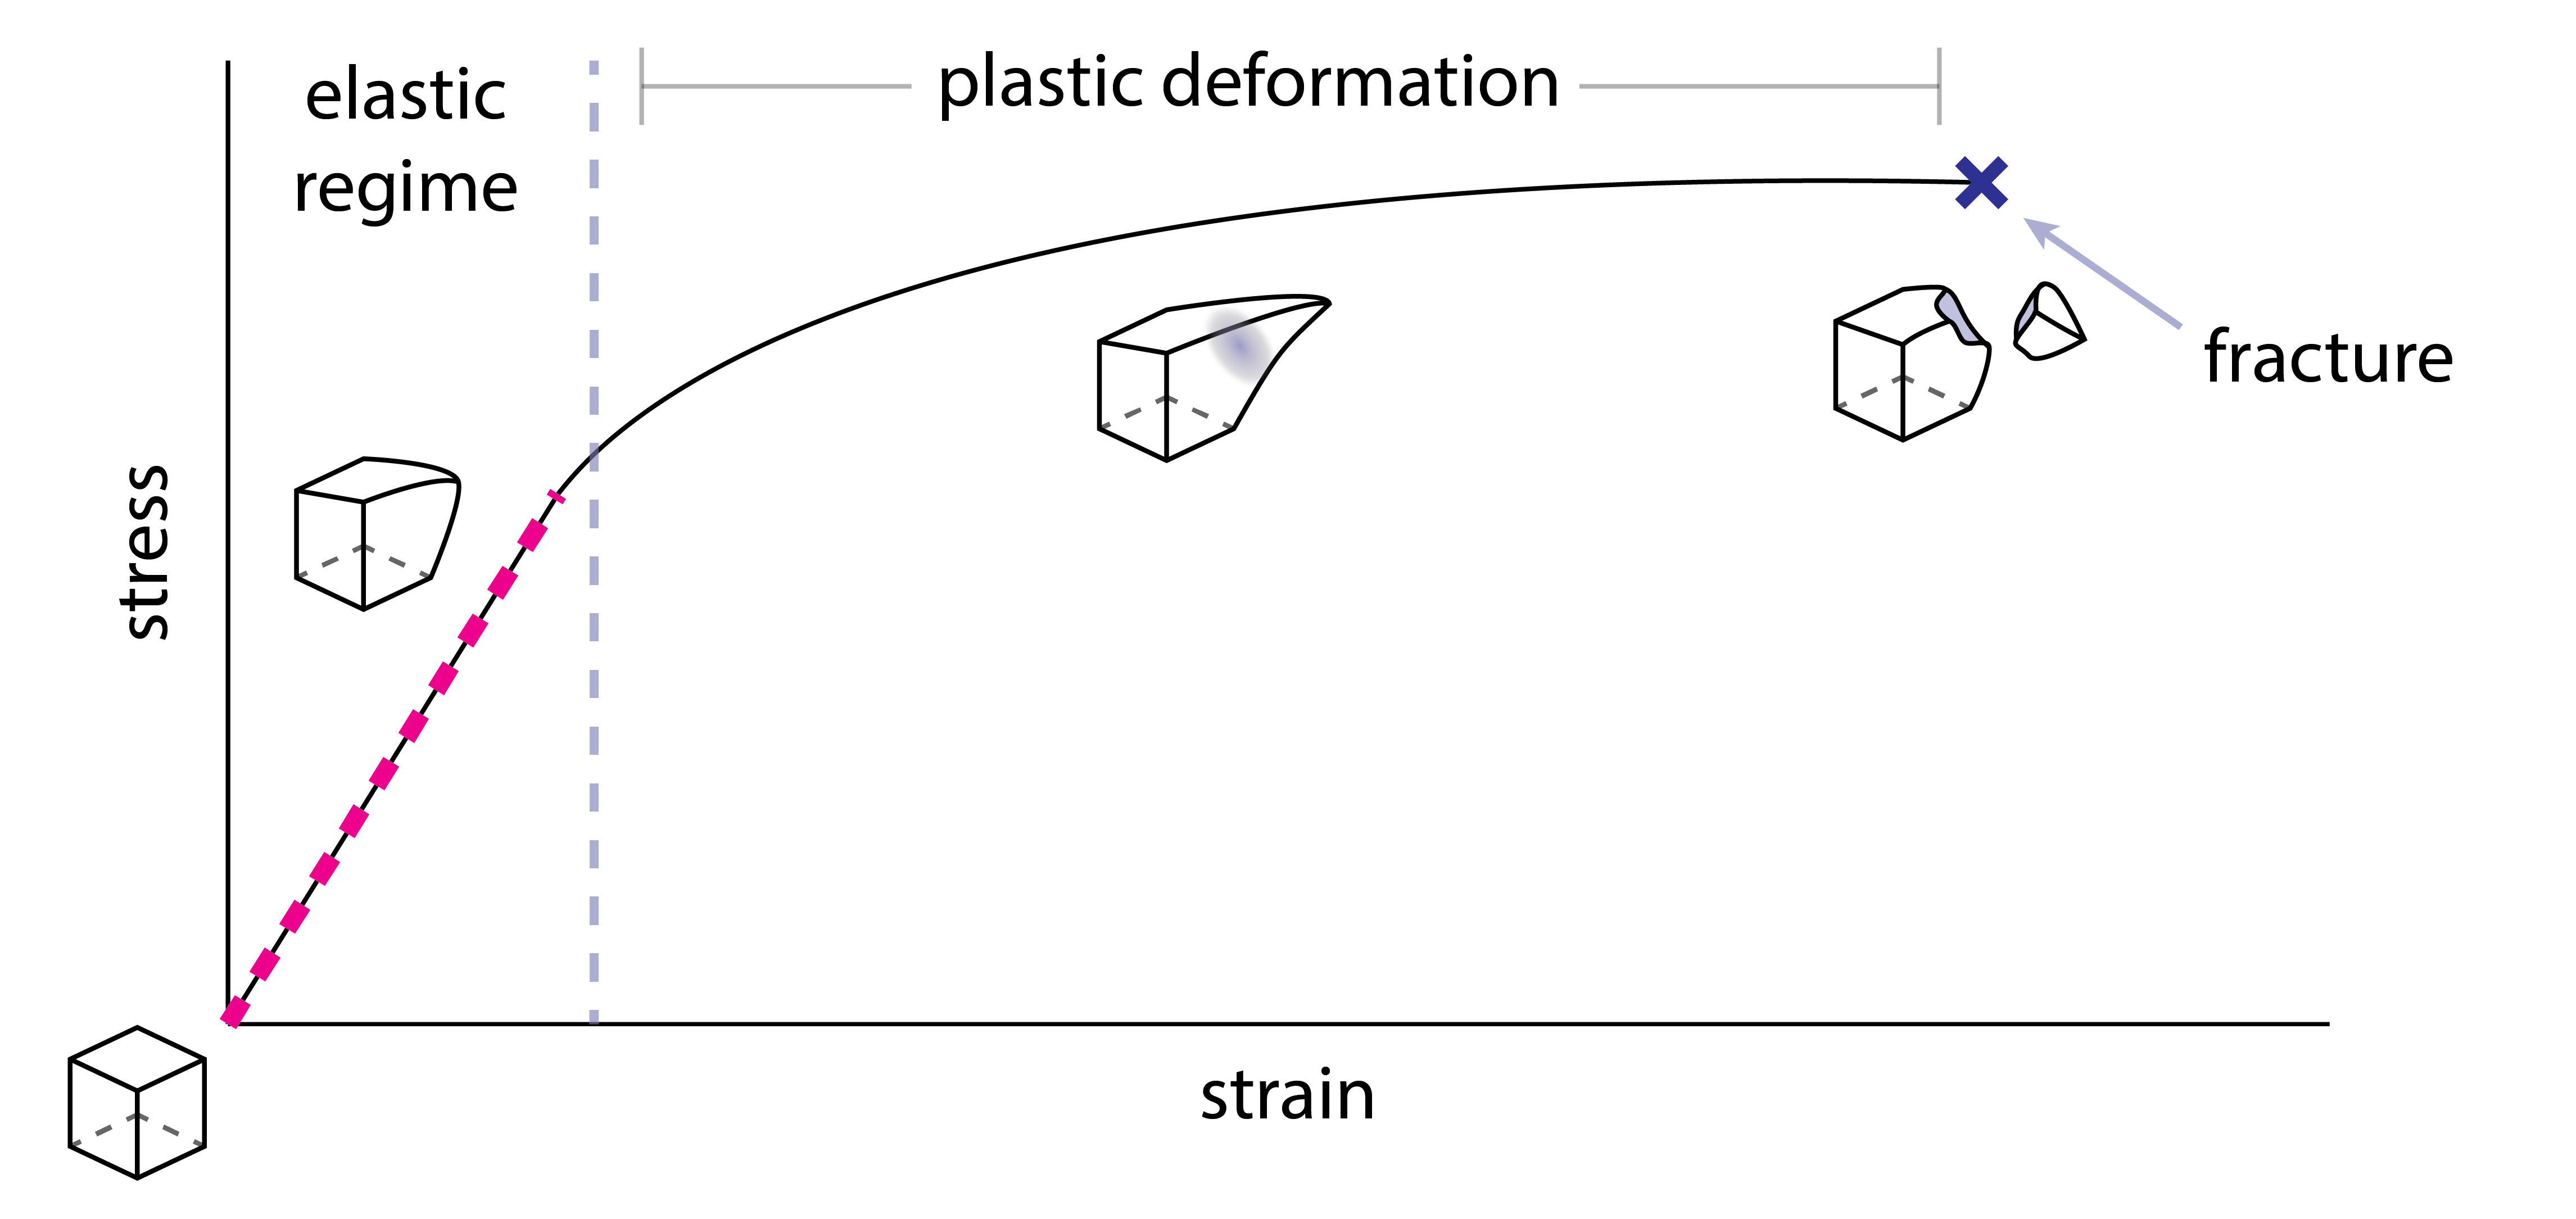
\includegraphics[width=\linewidth]{SolidRegimes.png}
  \caption{Stress/strain curves of materials reveal the linear elastic regime (pink), characterized by linear relationship between stress and strain and slope $E$ (elastic modulus).  Under larger stresses, materials enter non-linear elastic and plastic deformations, and eventually fracture.}
  \label{fig:SolidRegimes}
\end{figure}

The behavior of solids is typically characterized in terms of \textit{stress} and \textit{strain}.  Stress describes the internal forces acting on neighboring regions of a material, measured as force per area in pascals (Pa) or N/m\textsuperscript{2}.  Strain describes the deformations of these regions in response to stress, measured as a unit-less ratio of a length of deformation per unit of unstressed length.  Figure \ref{fig:SolidRegimes} shows an example of a typical stress/strain curve for a solid material.\\

Solids deform in an elastic regime until forces acting on or within them become so large they result in irreversible, plastic deformations or fracture (Figure \ref{fig:SolidRegimes}).  The modeling in this chapter will deal exclusively with \textit{linear} elastic deformations of solids.  This is the region of the stress/strain curve with constant slope, indicated by the pink dotted line in Figure \ref{fig:SolidRegimes}.  In this region, stress and strain have an approximately linear relationship to each other, in other words, materials obey Hooke's law:
\begin{equation}\label{eq:hookes}
F = kx
\end{equation}

where F is a force, x is a displacement, and k is a measure of geometeric stiffness.  We can rewrite Hooke's law in terms of stress ($\sigma$) and strain ($\epsilon$) as follows:
\begin{equation}\label{eq:stressstrain}
\sigma = E\epsilon 
\end{equation}

where $E$ is the elastic modulus (also called "Young's modulus") of a given material.  As long as the forces acting on and within a solid are sufficiently low, we can assume that a linear elastic deformation model applies.\\

\begin{figure}
  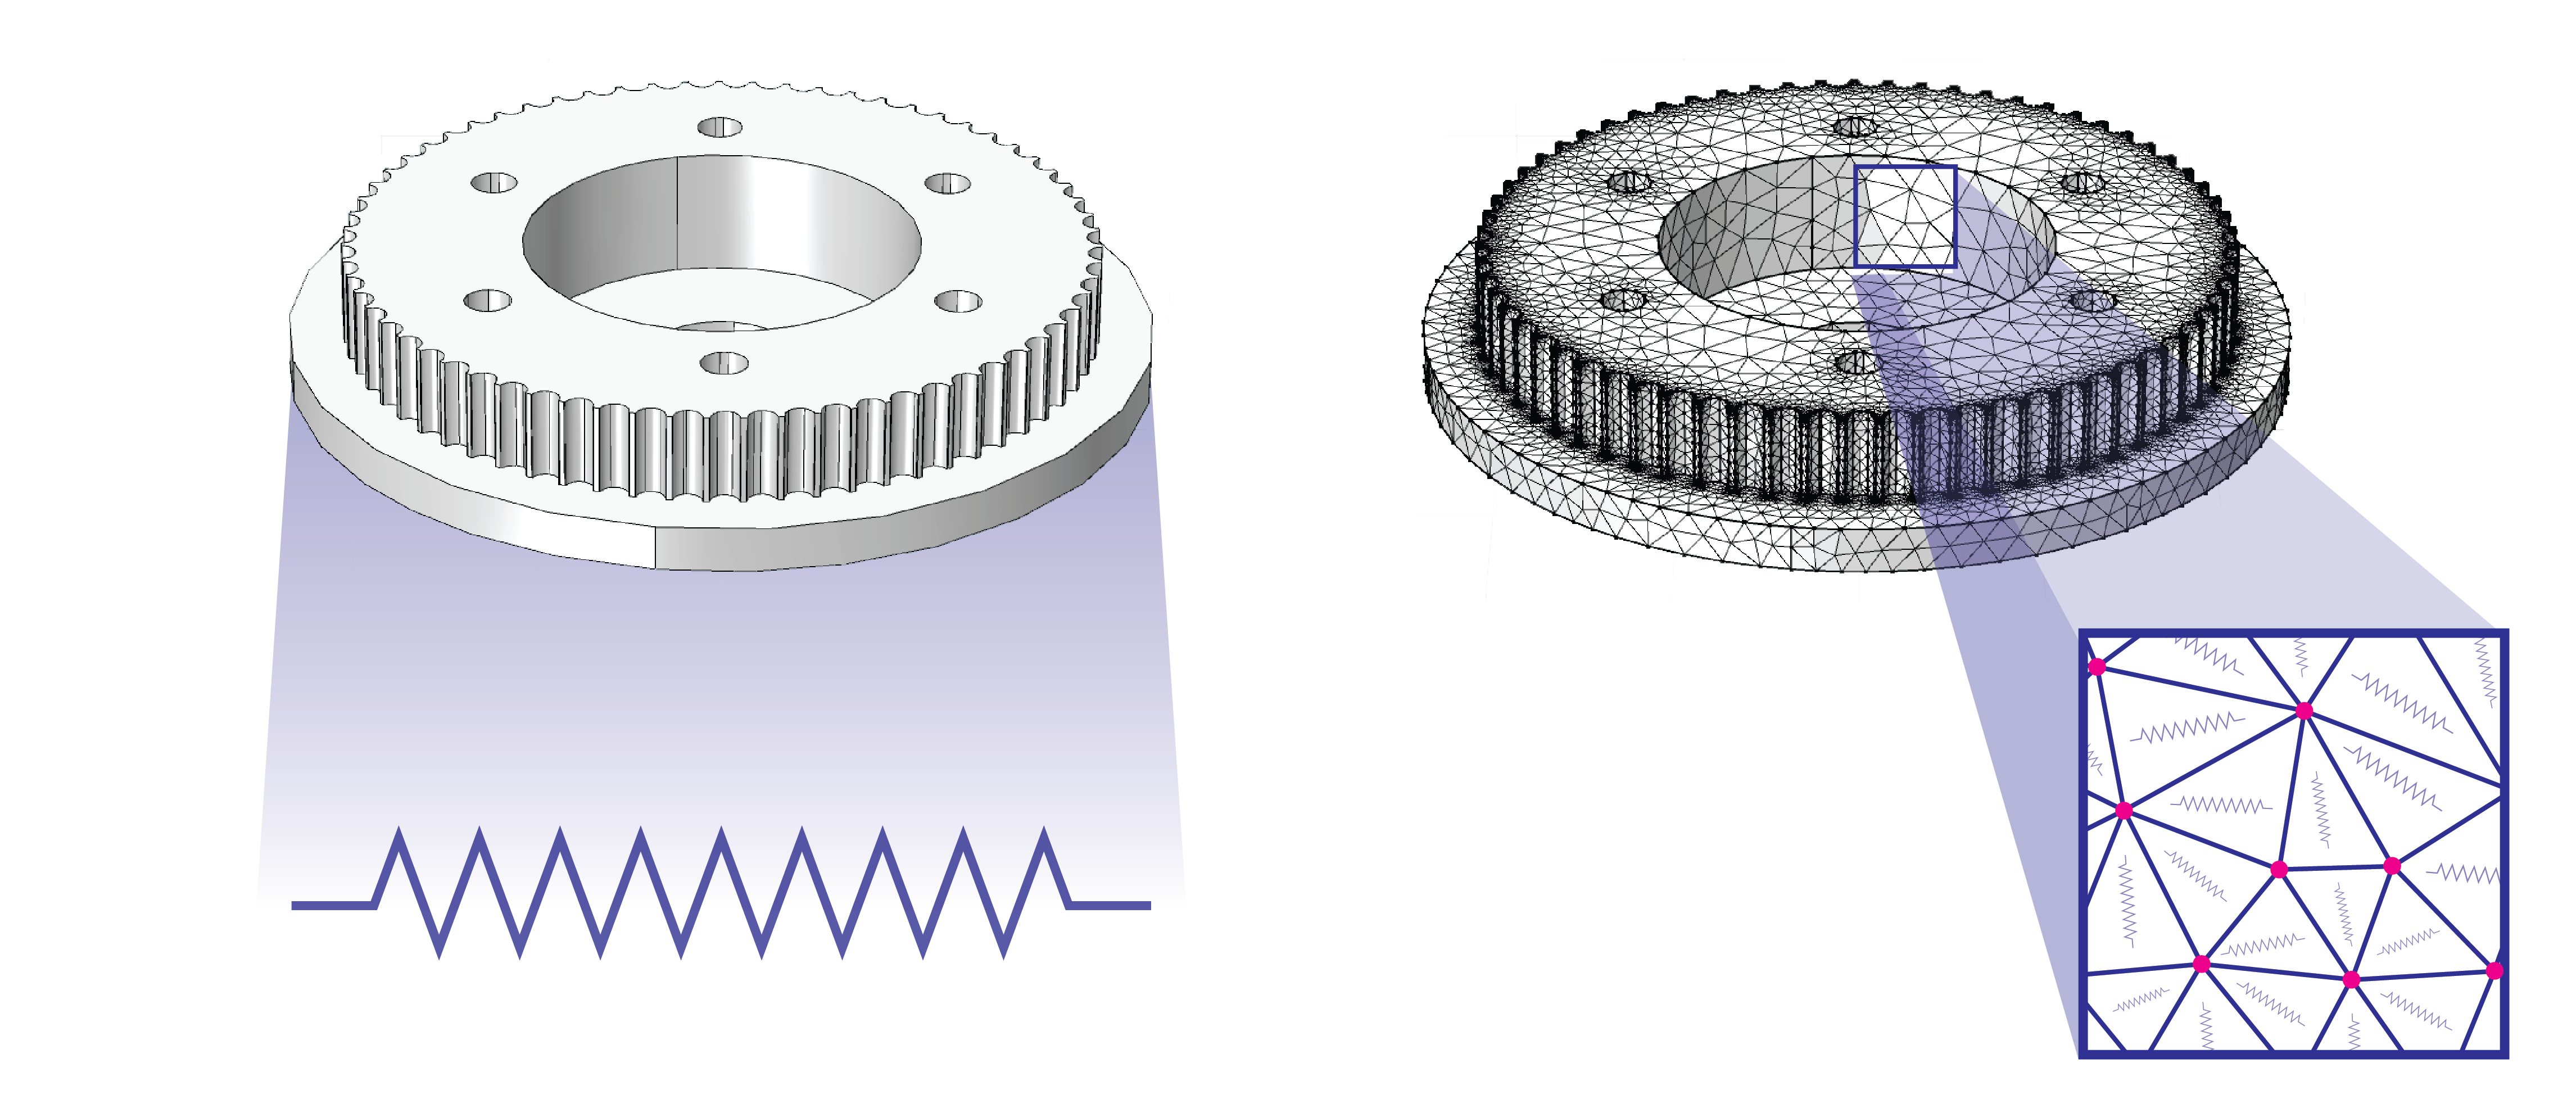
\includegraphics[width=\linewidth]{FEAexample.png}
  \caption{Two potential ways to model linear elastic deformations of a solid.  The strategy on the left treats the entire geometry as a Hookian spring, resulting in erroneous modeling of the solid's behavior.  The strategy on the left breaks up the solid into small regions which can individually be modeled with Hooke's law to a reasonable degree of accuracy.  The individual behaviors of the small regions are combined to synthesize a model of the global behavior of the entire geometry.  The method on the right summarizes the main idea behind traditional FEA.}
  \label{fig:FEAexample}
\end{figure}

So far we have discussed the ways that the material properties of a solid affect its behavior, next we must consider its geometry.  Starting with Equation \ref{eq:stressstrain}, we could try modeling the deformations of a linear, elastic solid as a single Hookian spring.  Though this strategy could yield reasonable results for simple geometries and loading patterns, like a rubberband in pure tension, it is not accurate for more complex situations.  Instead, modern simulation techniques break up complex geometries into many simple, discrete regions whose individual behavior can be accurately modeled with Hooke's law (Figure \ref{fig:FEAexample}).  Combining the solutions to these discrete regions approximates the net behavior of the more complex geometry.\\

Finite Element Analysis (FEA) is essentially the process of applying Hooke's law to many small regions of a geometry and adding up their result.\\


This thesis explores both isotropic and anisotropic materials.  A material is isotropic if it responds the same to an external force no matter its orientation; materials comprised of oriented fibers or other directional structures typical display anisotropic behaviors.  The response of solids to strains are typically expressed in terms of their elastic modulus $E$ and shear modulus $G$, however, for anisotropic materials, such as those used in our assembly system, this parameterization does not give enough information.\\







%This thesis is concerned with the numerical solution of the position, orientation, and deformation of an elastic solid made from many elements of identical geometry and various material types.  Evaluating this PDE subject to the initial state and boundary conditions (applied forces, fixed regions, etc) gives the state of the solid over time.


few works well for linear - non linear for large deformations may require remeshing\\
mass spring methods - widely used in computer graphics, better for large deformations and non linear, less accurate\\

Unlike traditional mass/spring/damper models of solids from computer graphics literature (cite stuff here), the model developed in this thesis draws on an abstraction of the functionality embedded in the different "function types".\\

\begin{figure}
  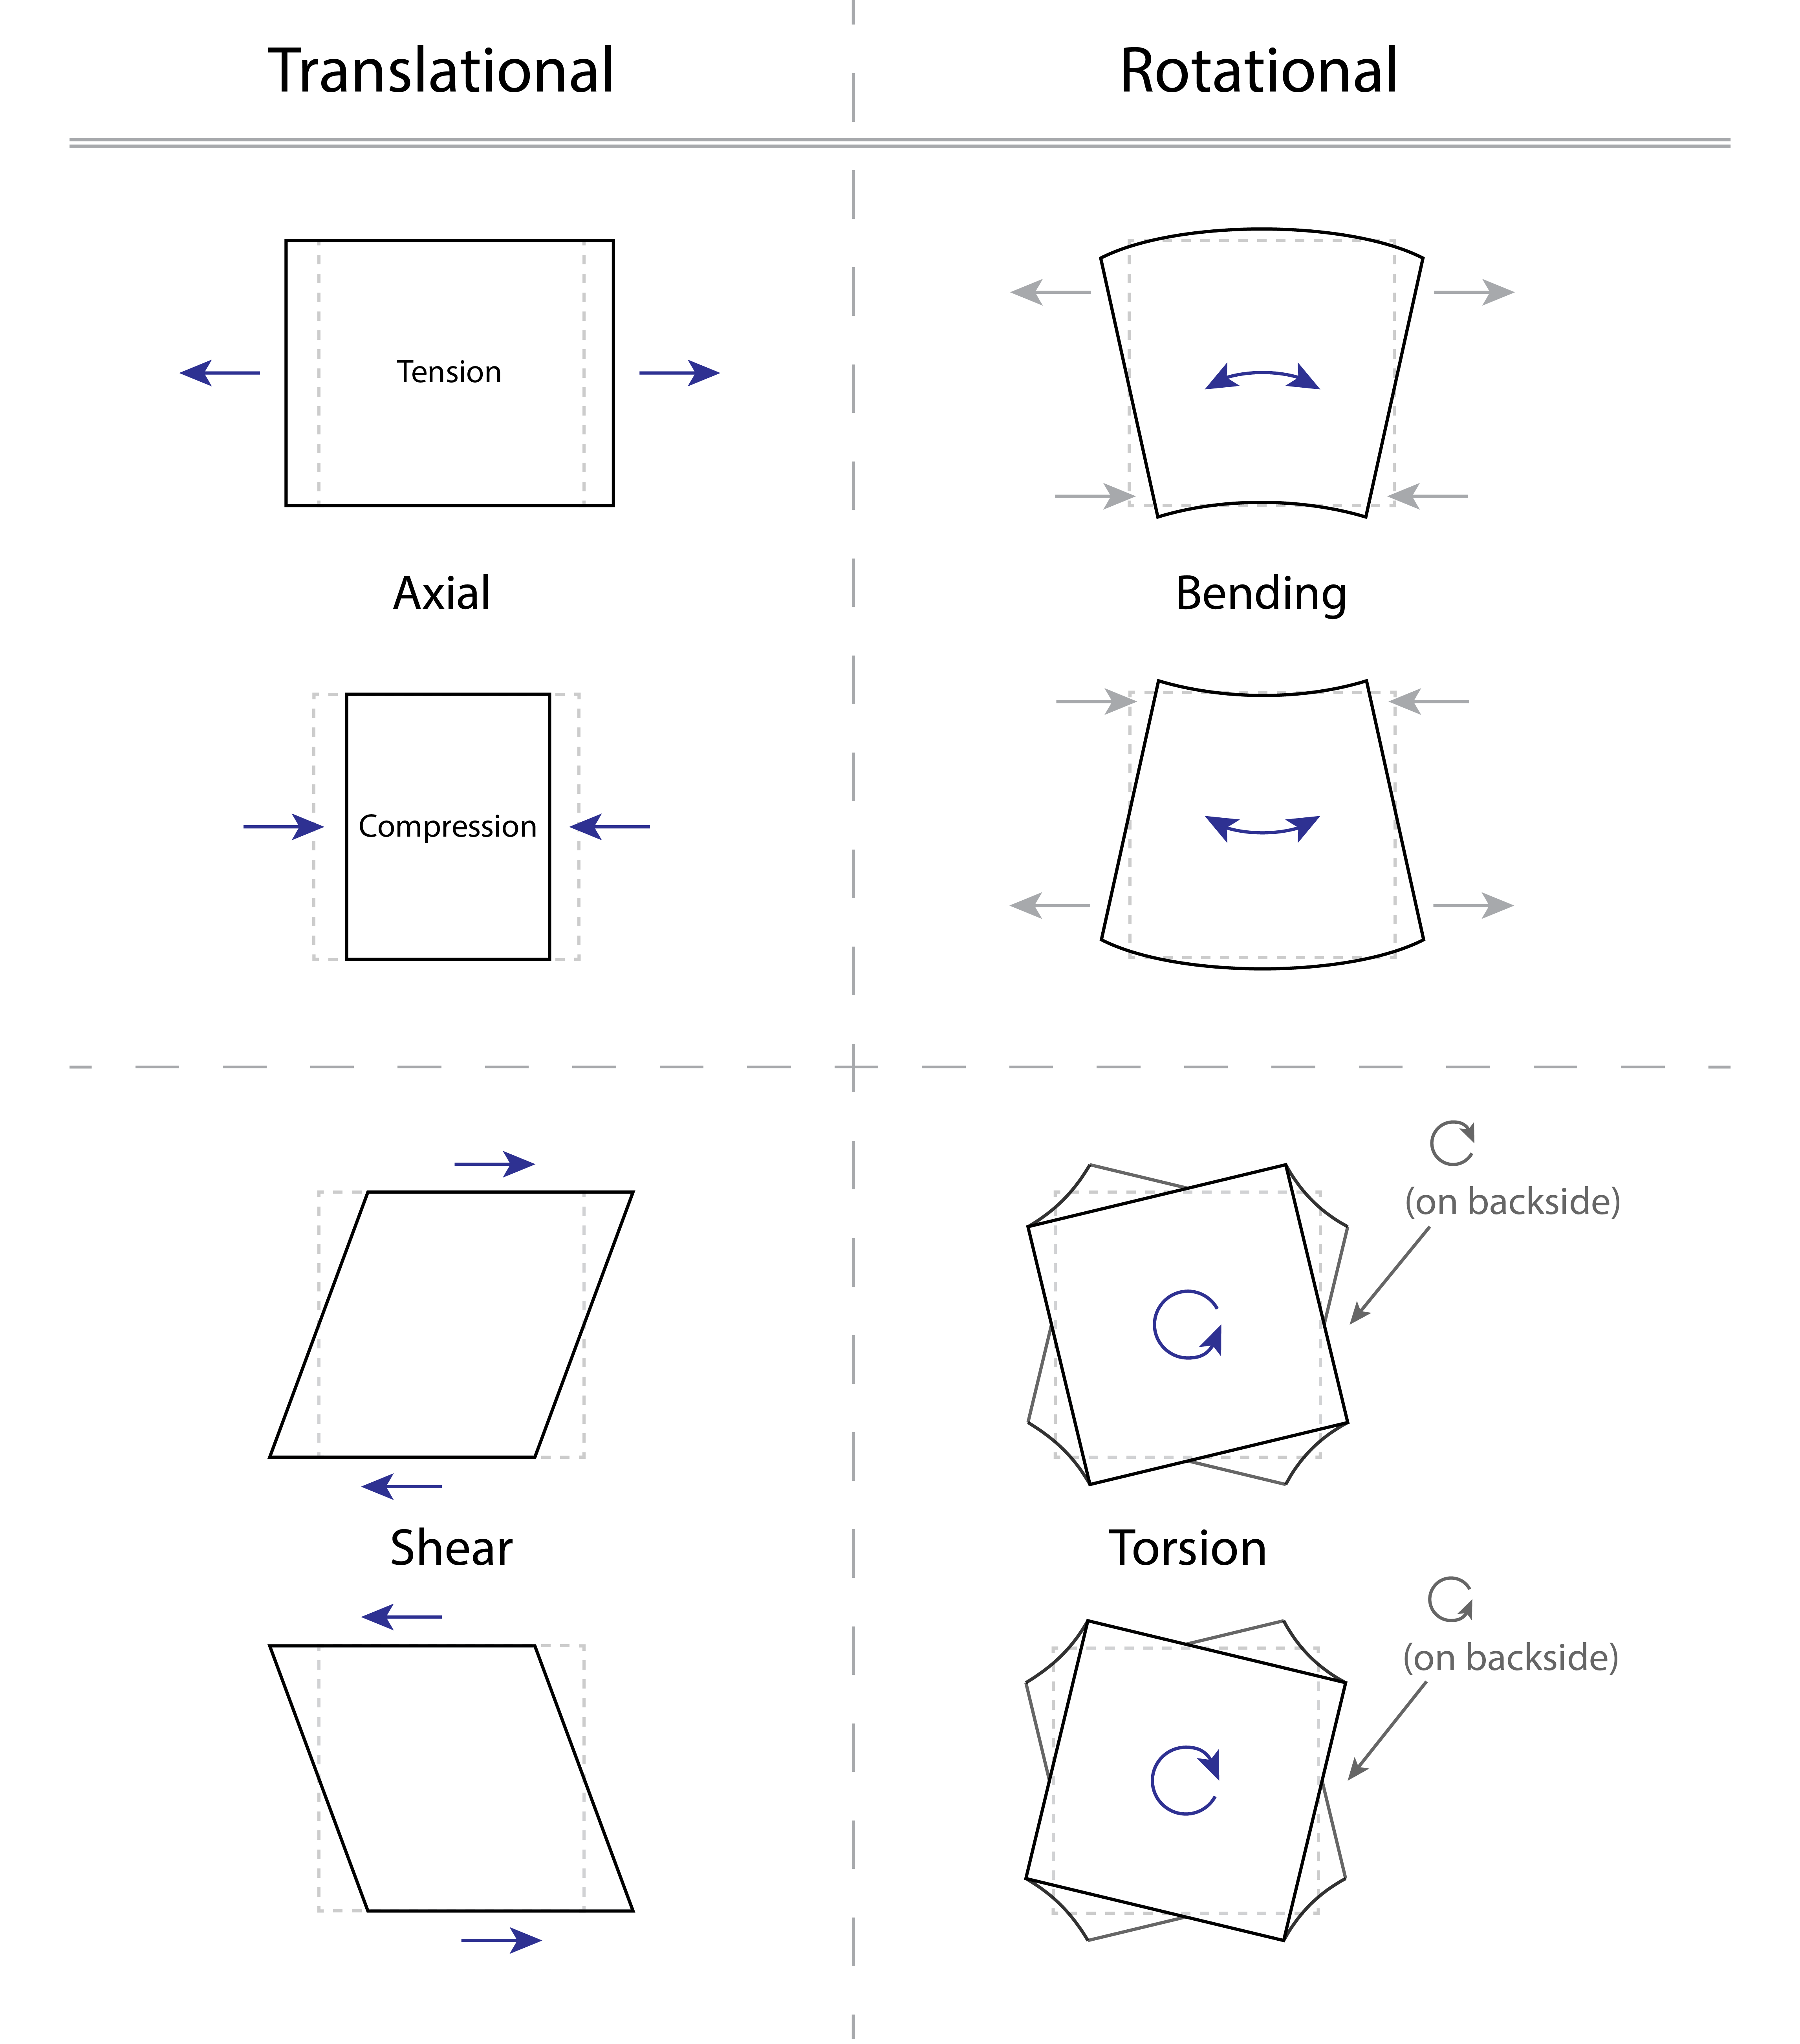
\includegraphics[width=\linewidth]{SolidMechanicsDOF.png}
  \caption{Deformations of a solid element under four types of applied forces.  In modeling assemblies of \textit{functions}, these characteristic deformations are referred to as "internal degrees of freedom".  Within an assembly of cells, axial (compression and tension) and shear forces cause translational displacement and bending and torsional forces cause rotational displacement.}
  \label{fig:SolidMechanicsDOF}
\end{figure}

In solid mechanics, we can consider the global deformations of a solid as the summation of deformations of many smaller, discrete volumes, or \textit{finite elements}.  Forces acting on these finite elements fall into four categories: axial (tension and compression), bending, shear, and torsion.  Each type of applied force causes a characteristic deformation of the finite element, illustrated in Figure \ref{fig:SolidMechanicsDOF}.  Applying multiple types of forces on a finite element will cause it to exhibit a combination of deformations.\\

In this model, simulation of an assembly happens at the granularity of identically-sized \textit{functional primitives}, which I'll call "cells" for the remainder of this chapter.  When describing mechanical behavior of a particular cell type, I'll refer to its deformations as "internal degrees of freedom" (DOF).  For example, a 1-DOF bending cell will have large deformations in bending along one axis, but relatively small deformations in response to other types of applied forces.\\

\section{Function Types}

\begin{figure}
  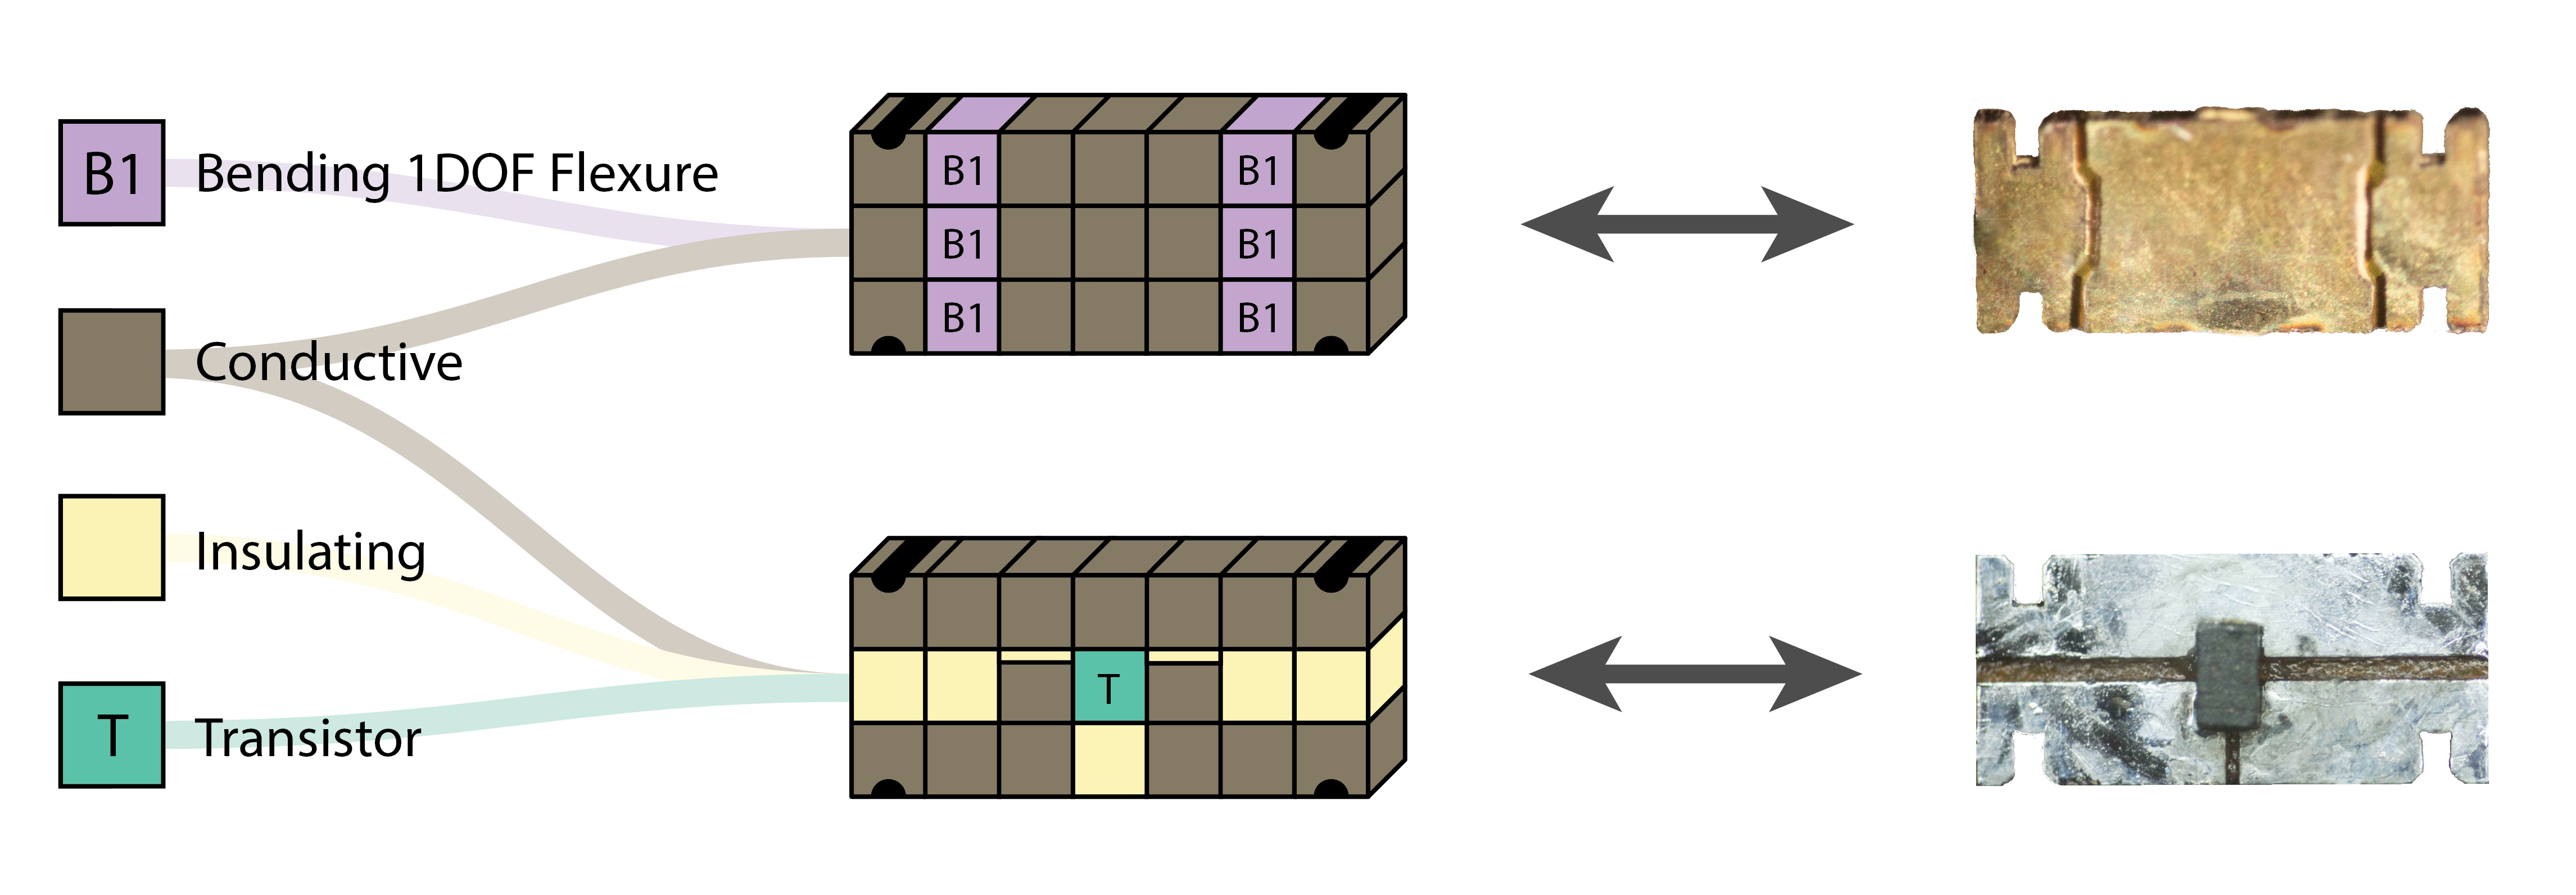
\includegraphics[width=\linewidth]{FunctionalPrimitives.png}
  \caption{}
  \label{fig:FunctionalPrimitives}
\end{figure}


Cells at the function-level are defined not only by their mechanical properties, but also by their ability to transmit electronic signals from one face to another, and their active properties in response to a signal. The combinatorial space of mechanical, electronic, and actuated cell types is described in Figure \ref{fig:CombinatoricsOfFunctions}.  Section \ref{sec:electronicSim} describes the process of electronic simulation in more detail, the remainder of this chapter will focus on the passive and active mechanical simulation of function-level cells.
\\

\begin{figure}
  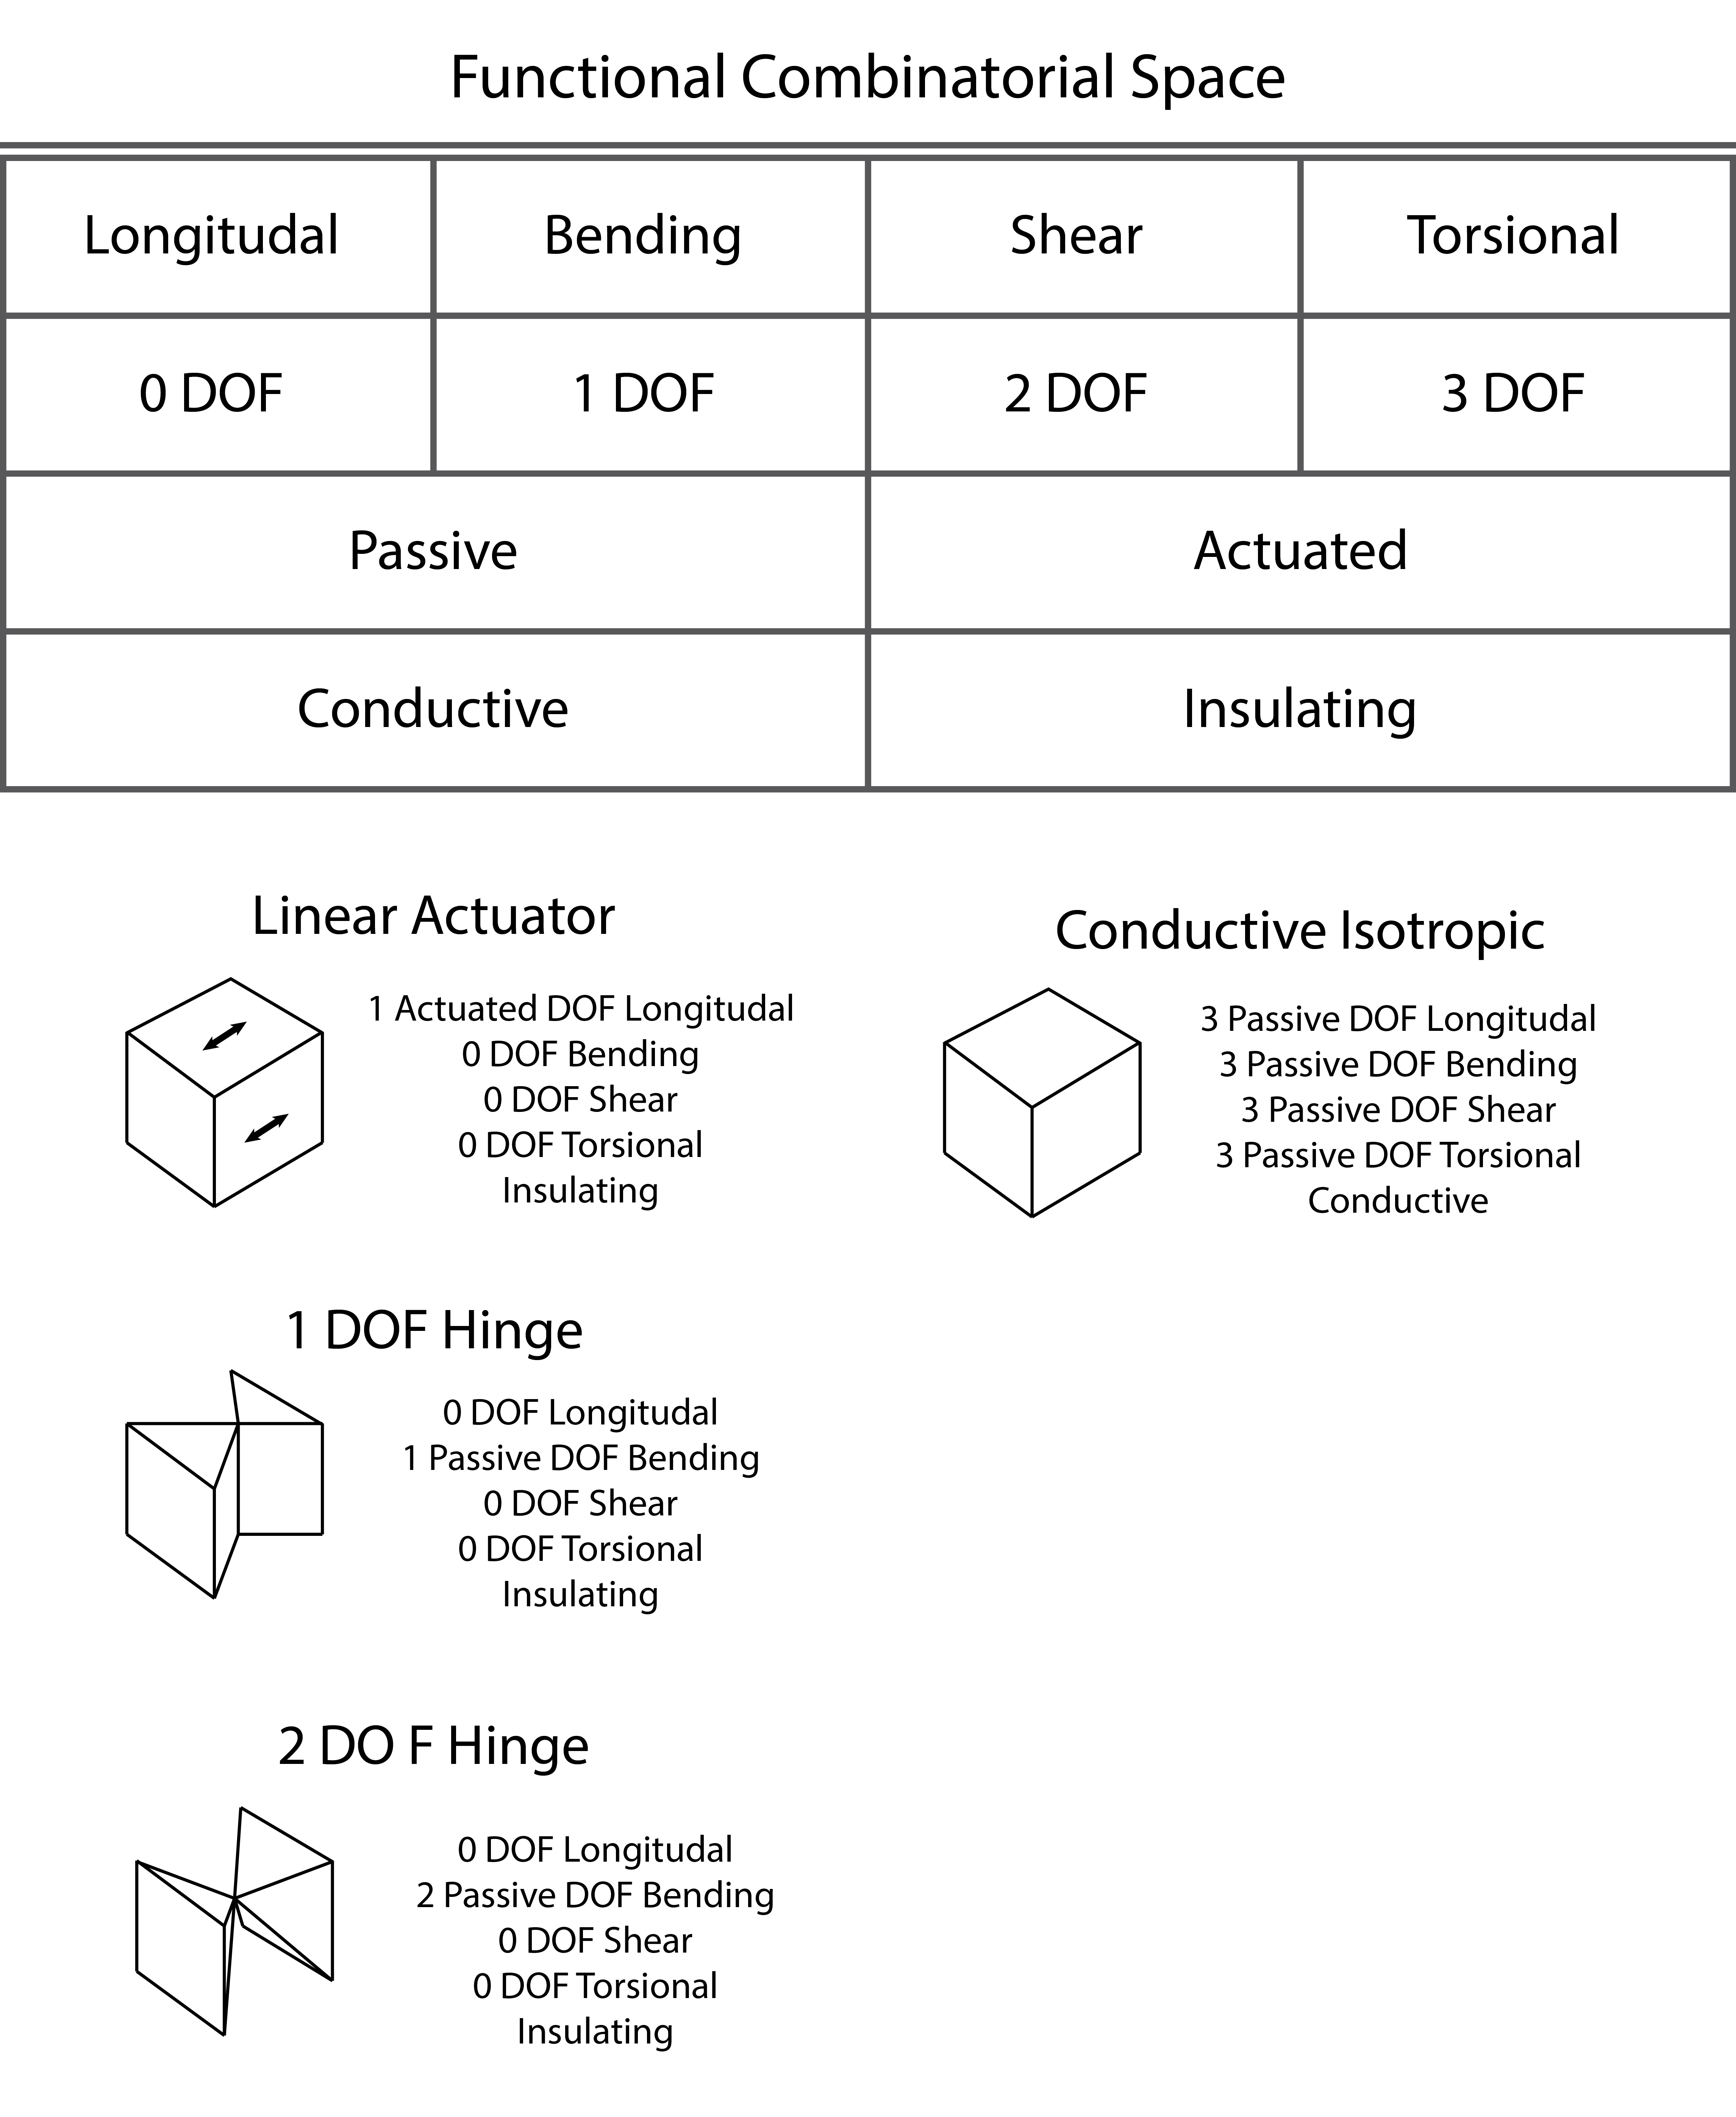
\includegraphics[width=\linewidth]{CombinatoricsOfFunctions.png}
  \caption{Combinatorial space of \textit{function} types with six examples explicitly described in terms of their electronic and mechanical properties.  Note - any individual degree of freedom within a cell falls on the spectrum described in Figure \ref{fig:BendingStiffnessContinuoum}.  A cell is described at a high level as having a particular degree of freedom if its corresponding stiffness in that dimension is sufficiently flexible to allow for significant deformation uder applled load.  There are no infinitely stiff or fully unconstrained degrees of freedom in this system.}
  \label{fig:CombinatoricsOfFunctions}
\end{figure}

A linear scale showing the range of physically achievable 1-DOF bending cell types compared with the range of theoretically possible types is shown in Figure \ref{fig:BendingStiffnessContinuoum}.  Due to manufacturing and material constraints, we do not envision \textit{function}-level cells that occupy the region near zero bending stiffness (e.g. a frictionless pin joint) or infinite bending stiffness (zero compliance material).

\begin{figure}
  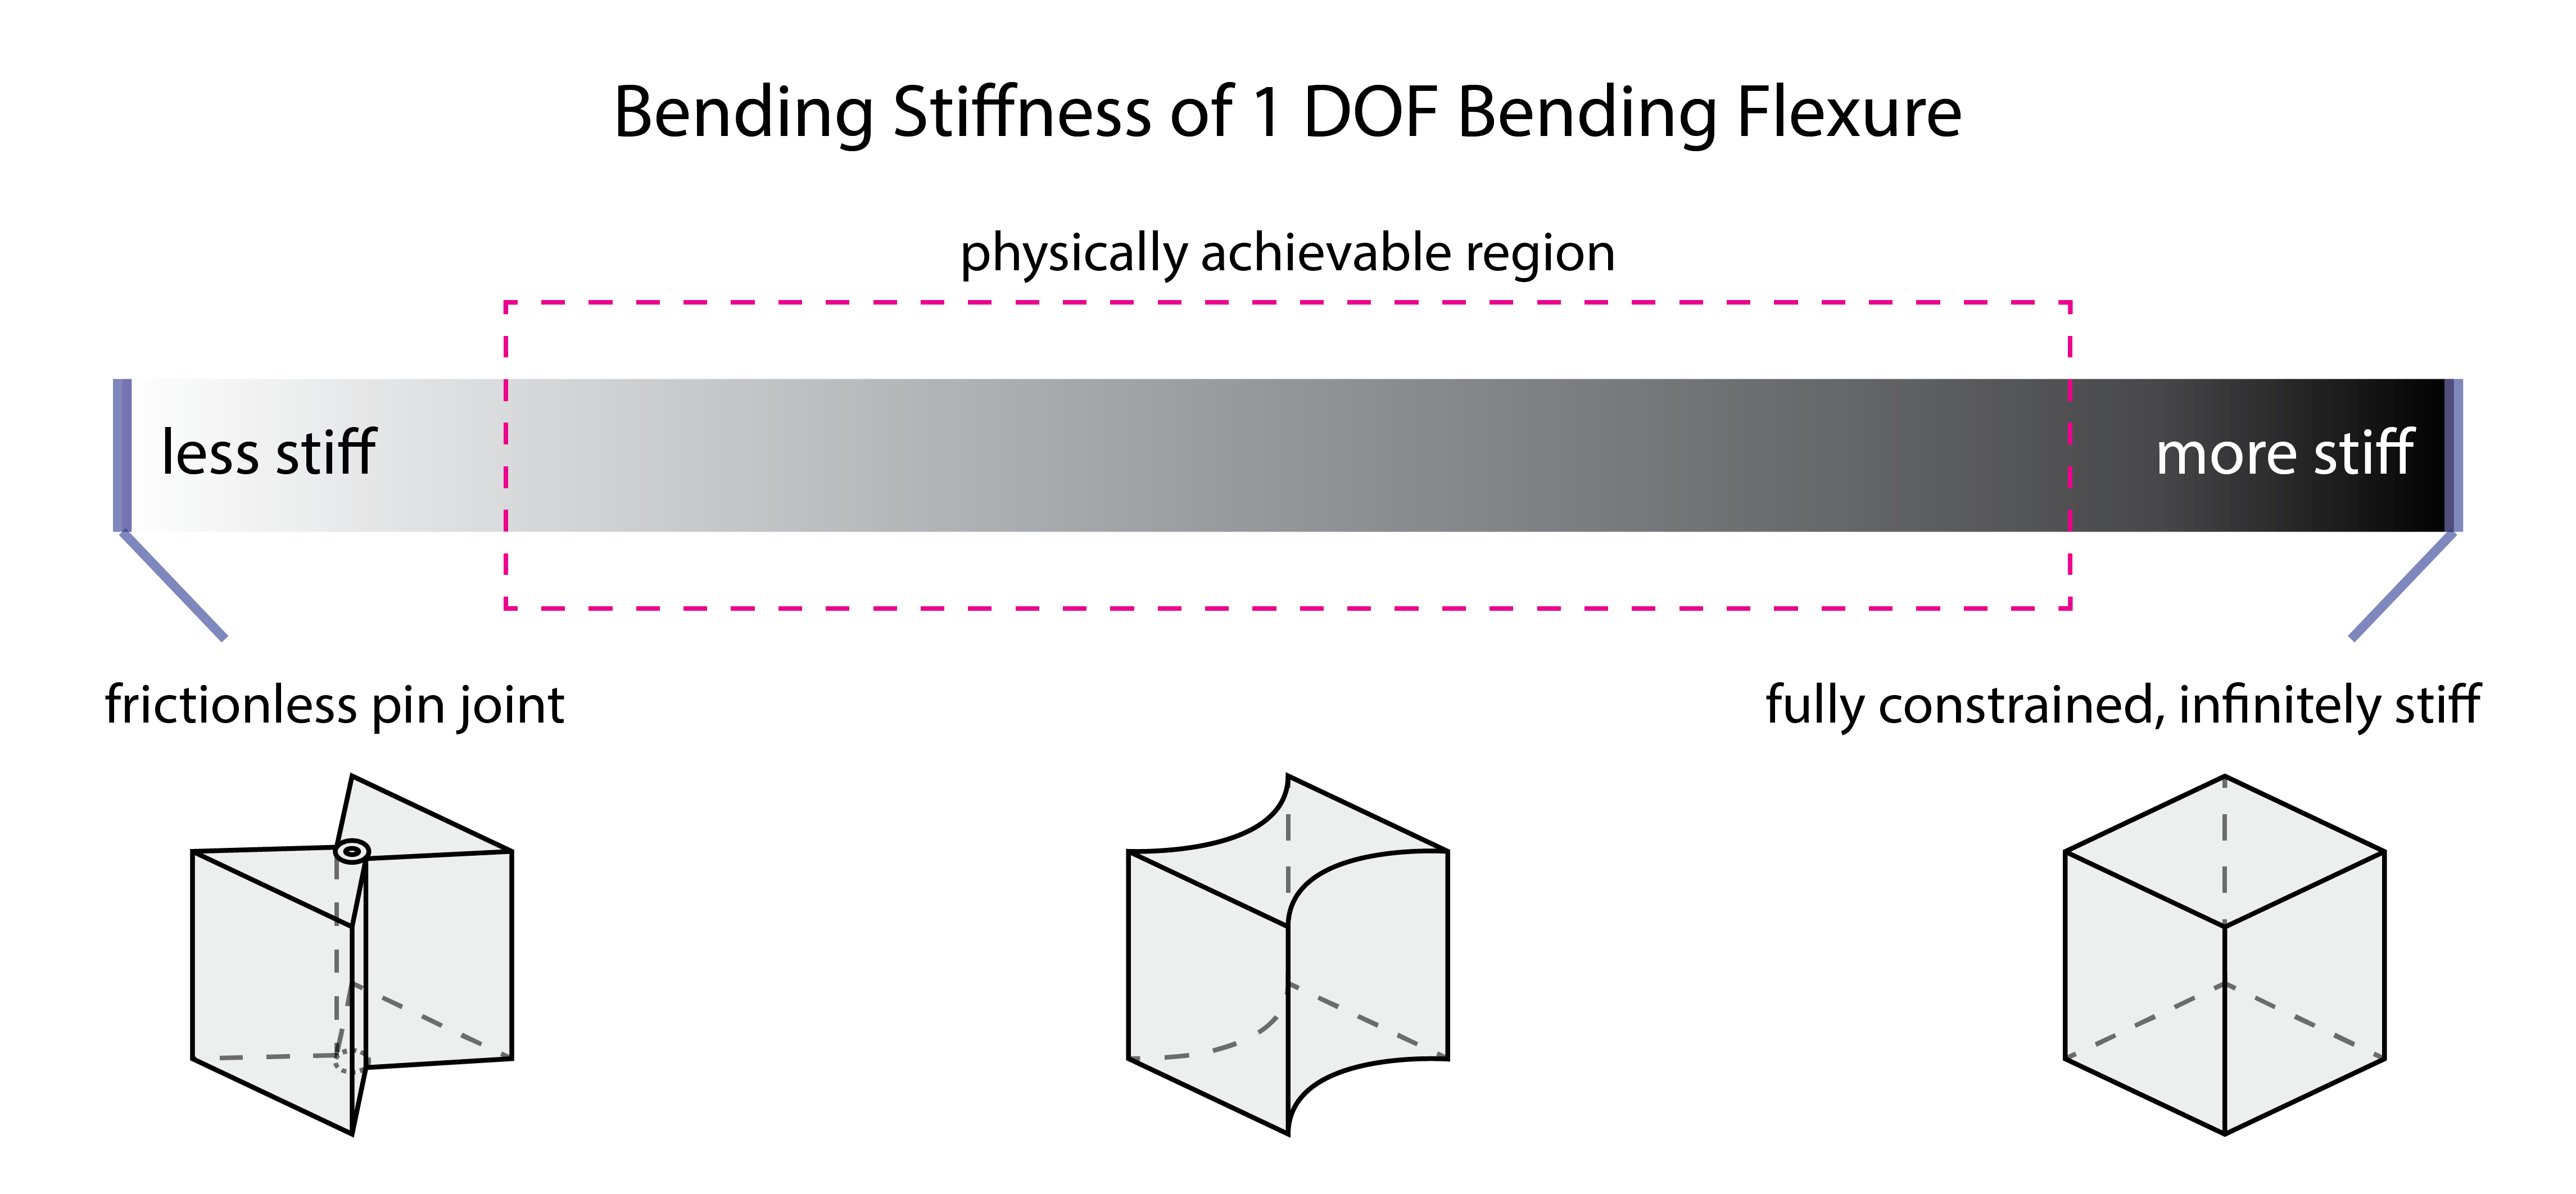
\includegraphics[width=\linewidth]{BendingStiffnessContinuoum.png}
  \caption{Continuum of bending stiffness in a 1 DOF hinge.}
  \label{fig:BendingStiffnessContinuoum}
\end{figure}

\section{Spring-Damper Characteristics}

The geometric stiffness of a structure relates the bulk properties of a material to its 3d geometry.  For example, an I-beam has a higher geometric bending stiffness than an equal length rectangular bar made from the same amount of the same material.  Unless otherwise noted, "stiffness" in this analysis refers to geometric stiffness.\\

Stiffness and damping are used to characterize the response of cell's internal degrees of freedom to applied external forces.  Stiffness has the units N/m and damping N$\cdot$s/m.  In three dimensions, each cell's passive mechanical properties are parameterized by 15 stiffness and damping constants:

\[ k  = \begin{cases}
\enspace k_{axial_x}\\
\enspace k_{axial_y}\\
\enspace k_{axial_z}\\
\\
\enspace k_{shear_{xy}}\\
\enspace k_{shear_{xz}}\\
\enspace k_{shear_{yx}}\\
\enspace k_{shear_{yz}}\\
\enspace k_{shear_{zx}}\\
\enspace k_{shear_{zy}}\\
\\
\enspace k_{bending_x}\\
\enspace k_{bending_y}\\
\enspace k_{bending_z}\\
\\
\enspace k_{torsional_x}\\
\enspace k_{torsional_y}\\
\enspace k_{torsional_z}
 \end{cases}
 \qquad\qquad
 d  = \begin{cases}
\enspace d_{axial_x}\\
\enspace d_{axial_y}\\
\enspace d_{axial_z}\\
\\
\enspace d_{shear_{xy}}\\
\enspace d_{shear_{xz}}\\
\enspace d_{shear_{yx}}\\
\enspace d_{shear_{yz}}\\
\enspace d_{shear_{zx}}\\
\enspace d_{shear_{zy}}\\
\\
\enspace d_{bending_x}\\
\enspace d_{bending_y}\\
\enspace d_{bending_z}\\
\\
\enspace d_{torsional_x}\\
\enspace d_{torsional_y}\\
\enspace d_{torsional_z}
 \end{cases}  \]
\\

$k_{shear}$ and $d_{shear}$ are broken out into six parameters of the form $shear_{nm}$ because the shear response depends both on the direction of shear displacement between two cells ($m$) and on the axis along which the cells are connected ($n$).  The $shear_{nm}$ notion used above is described graphically in in Figure \ref{fig:ShearDOFs}.\\

\begin{figure}
  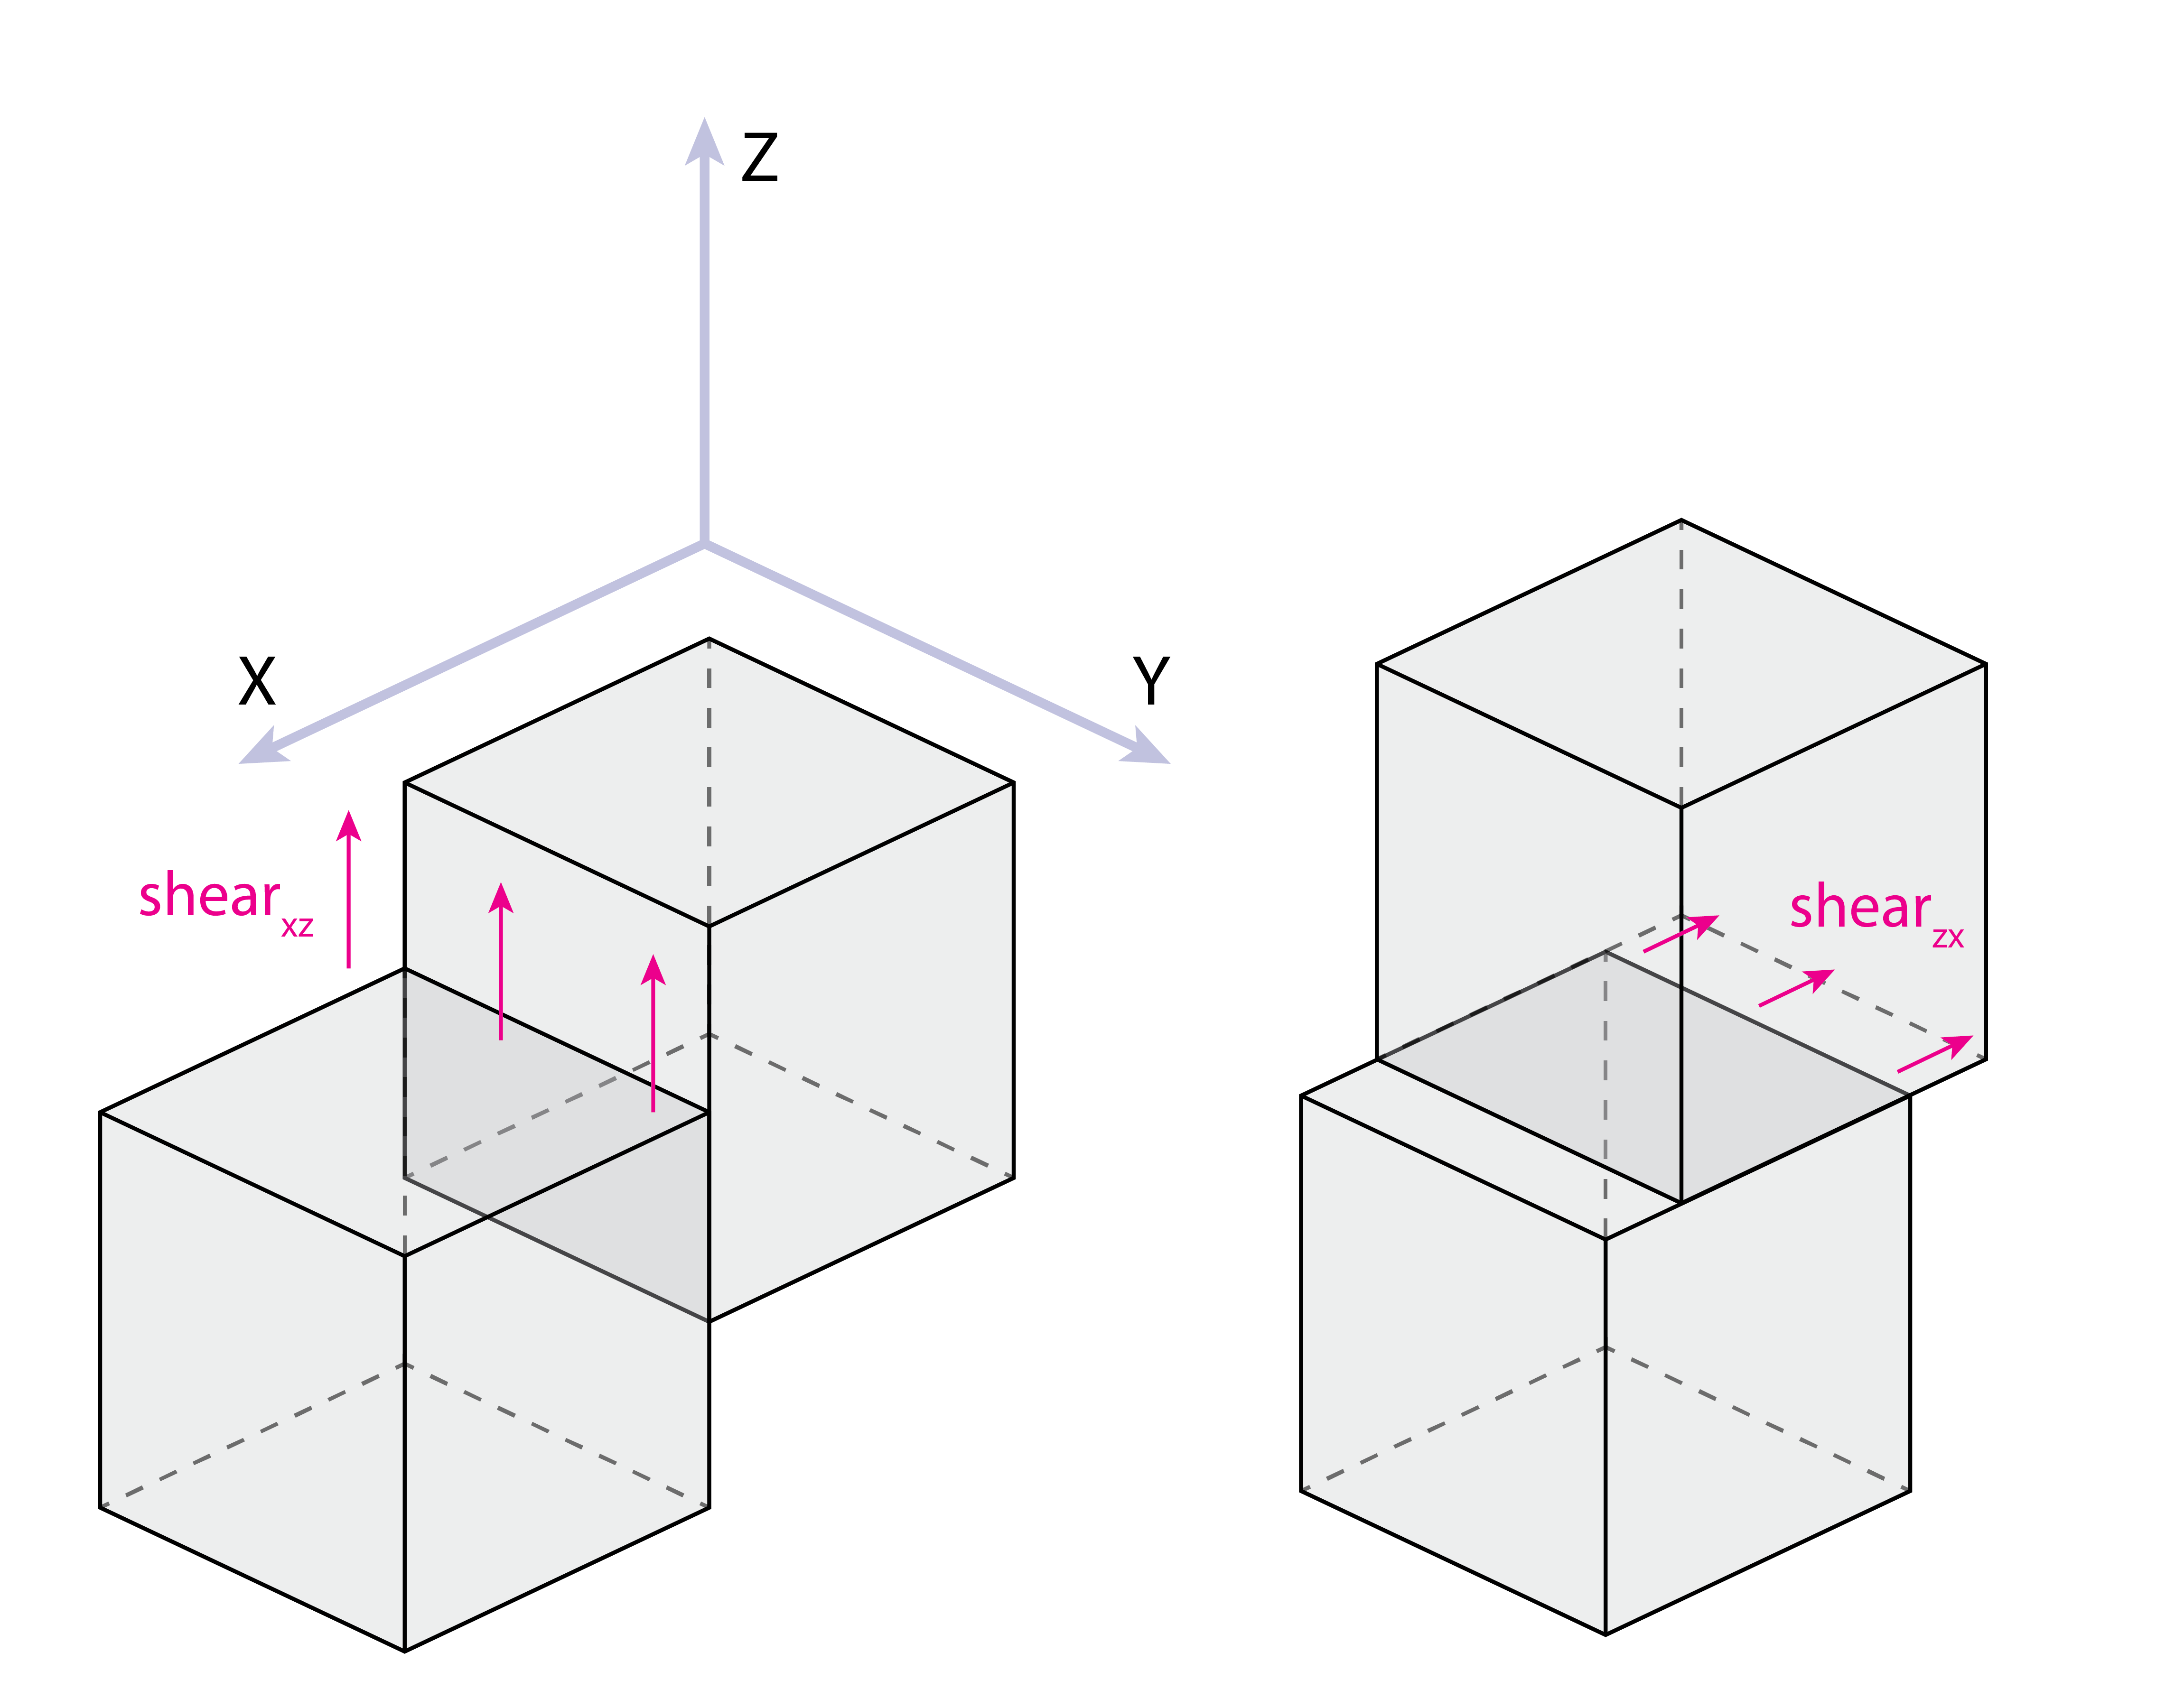
\includegraphics[width=\linewidth]{ShearDOFs.png}
  \caption{Illustration of shear subscript notation.  First subscript describes the direction of neighboring cell connection, second describes the direction of shear displacement.}
  \label{fig:ShearDOFs}
\end{figure}`	1

The stiffness and damping constants of each cell type may be calculated from bulk properties of the constituent materials that make up the cell, or they may be measured empirically.  For example, an isotropic cell made from a bulk material with elastic modulus $E$ and shear modulus $G$ has stiffnesses defined by:

\begin{subequations}
\begin{align} 
\label{eq:kaxial}
k_{axial} &= \dfrac{aE}{l}\\[10pt]
\label{eq:kshear}
k_{shear} &= \dfrac{3EI}{al}\\[10pt]
\label{eq:ktorsion}
k_{torsion} &= \dfrac{GJ}{l}\\[10pt]
\label{eq:kbending}
k_{bending} &= \dfrac{EI}{l}
\end{align}
\end{subequations}
\\
where $a$ is the cross sectional area and $l$ is the length of the cell.\\

 In the case that the cells have different stiffness or damping constants, a composite stiffness or damping constant must be calculated in order to properly model the junction between the cells.  Composite stiffness can be calculated according to the following formula:
 \begin{equation} \label{eq:springseries}
 k_{composite} = \dfrac{2k_1k_2}{k_1+k_2}
 \end{equation}

similarly, composite damping is calculated by:
 \begin{equation} \label{eq:damperseries}
d_{composite} = \dfrac{2d_1d_2}{d_1+d_2}
 \end{equation}
 
 Equations \ref{eq:springseries} and \ref{eq:damperseries} are equivalent to the formulas for two springs or two dampers of half length in series.  This is demonstrated graphically in Figure \ref{fig:SeriesCoupling}.  Notice, for example, in the case of $k1=k2$, Equation \ref{eq:springseries} reduces to $ k_{composite} = k1 = k2$.\\
 
 \begin{figure}
  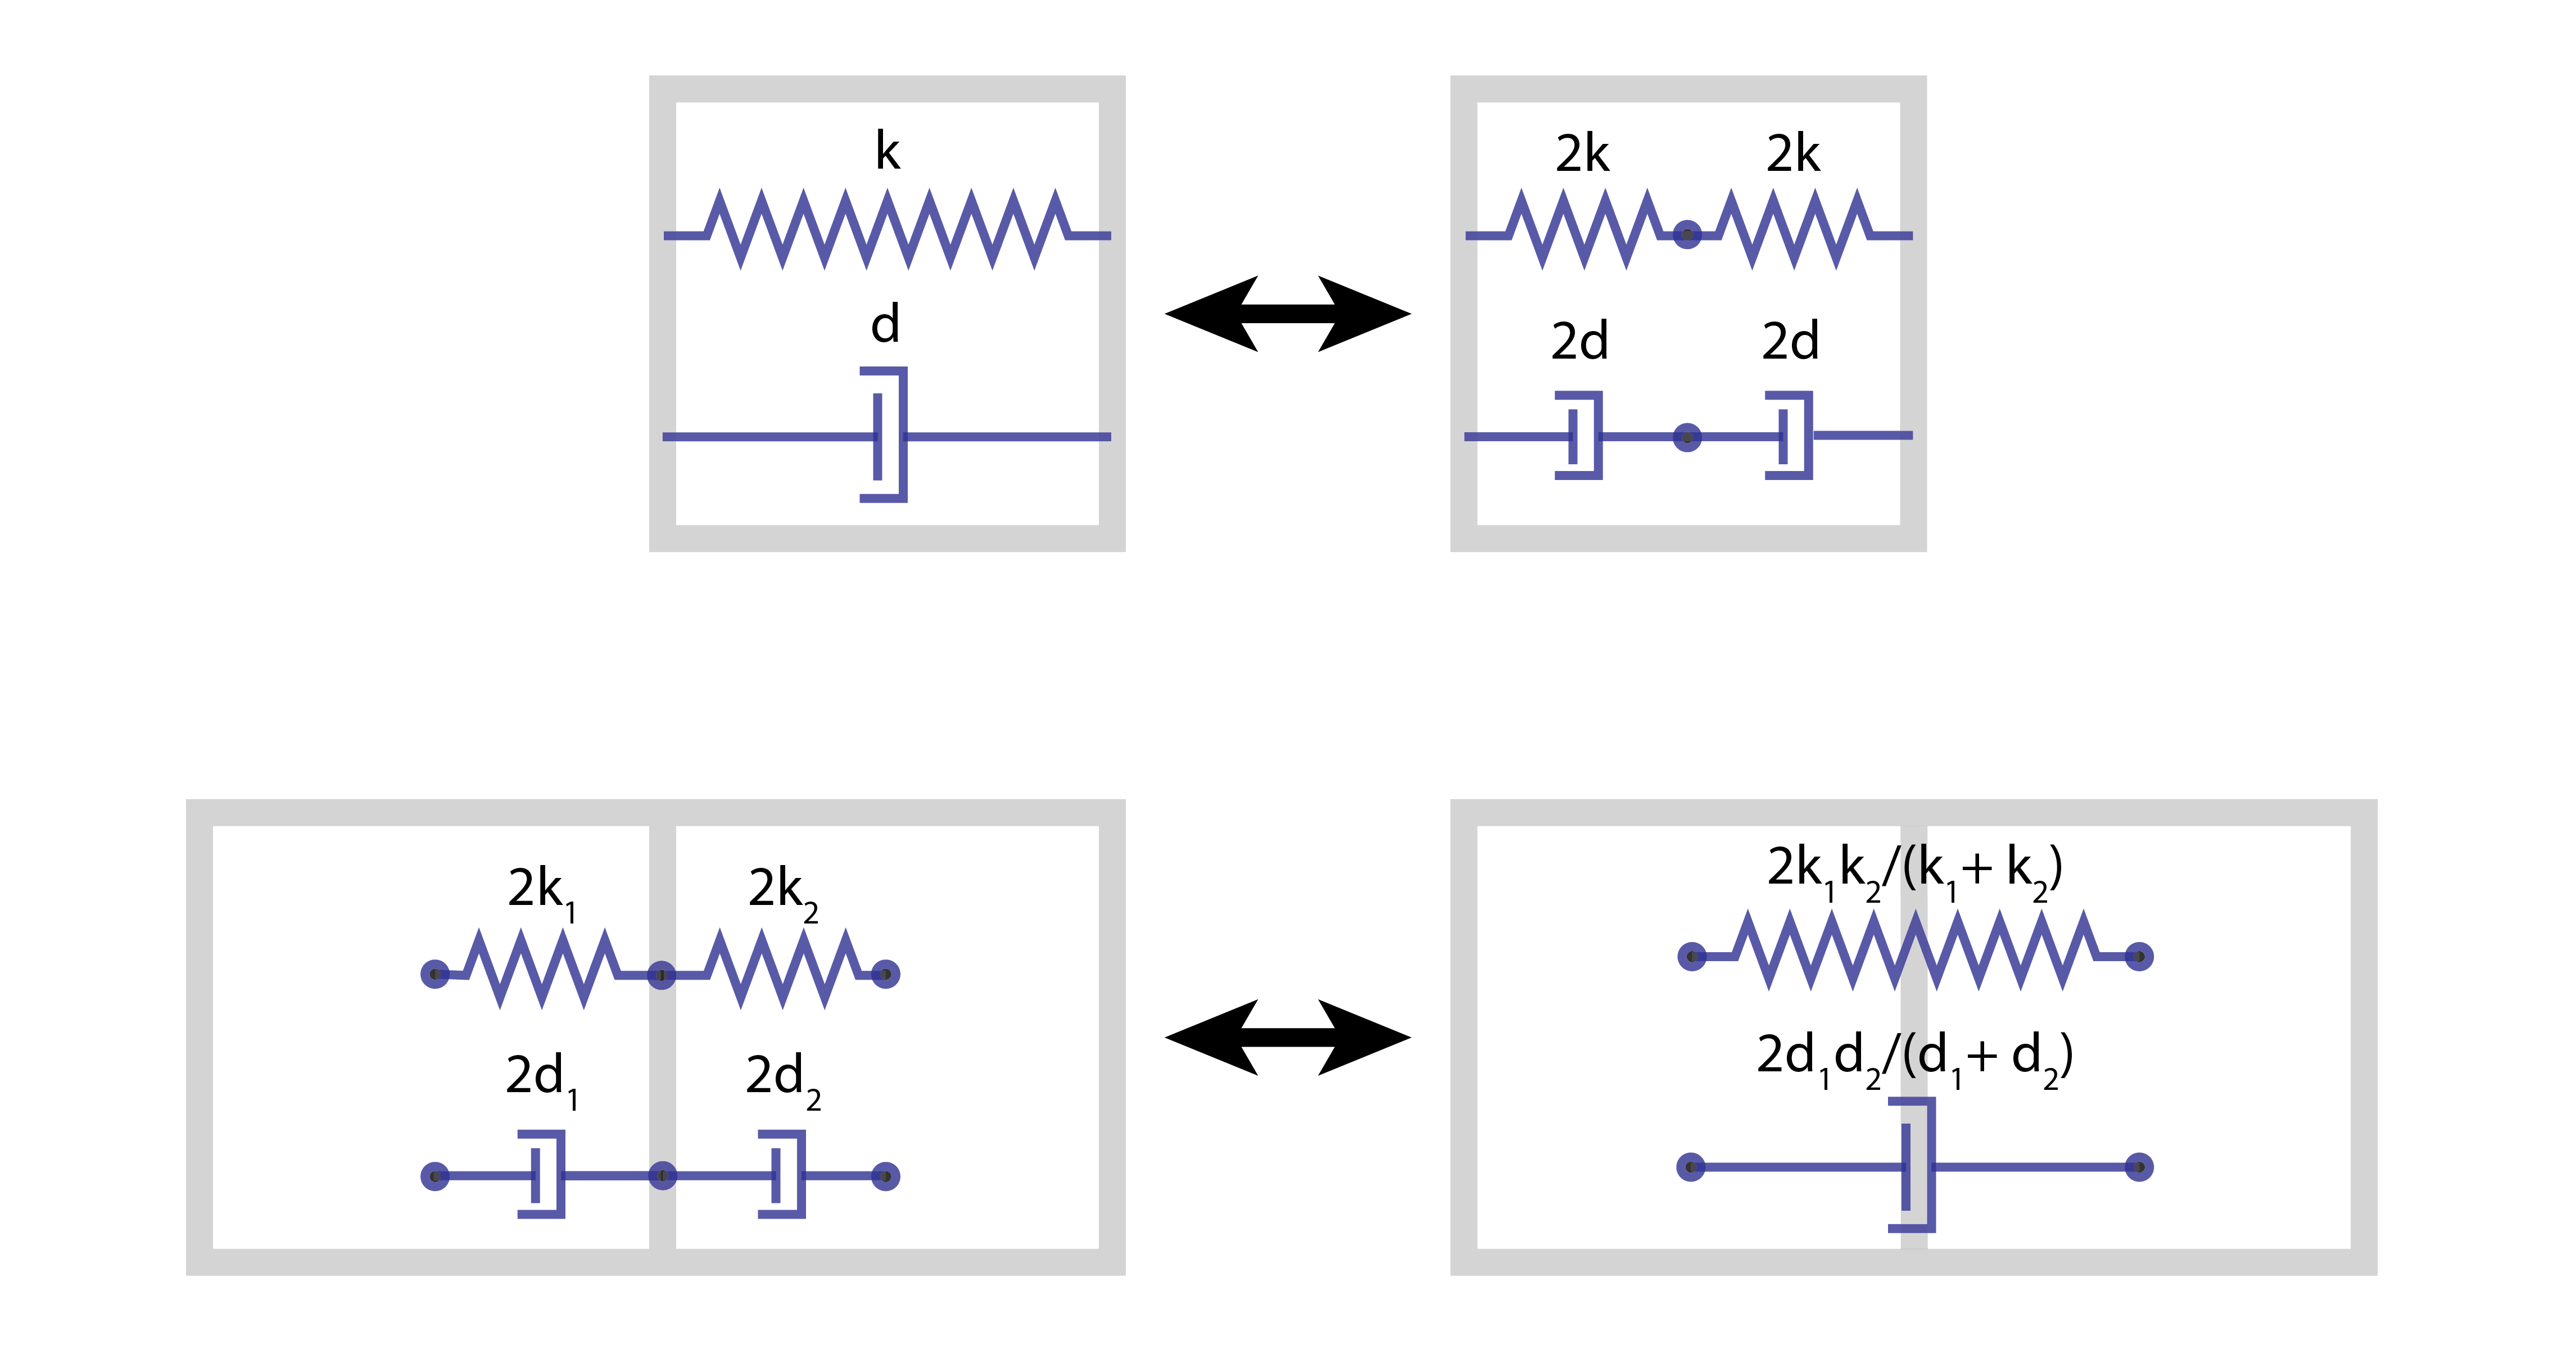
\includegraphics[width=\linewidth]{SeriesCoupling.png}
  \caption{Calculation of composite stiffness and damping of two cells with different k and d constants.}
  \label{fig:SeriesCoupling}
\end{figure}


\section{Translational Forces}

\begin{figure}
  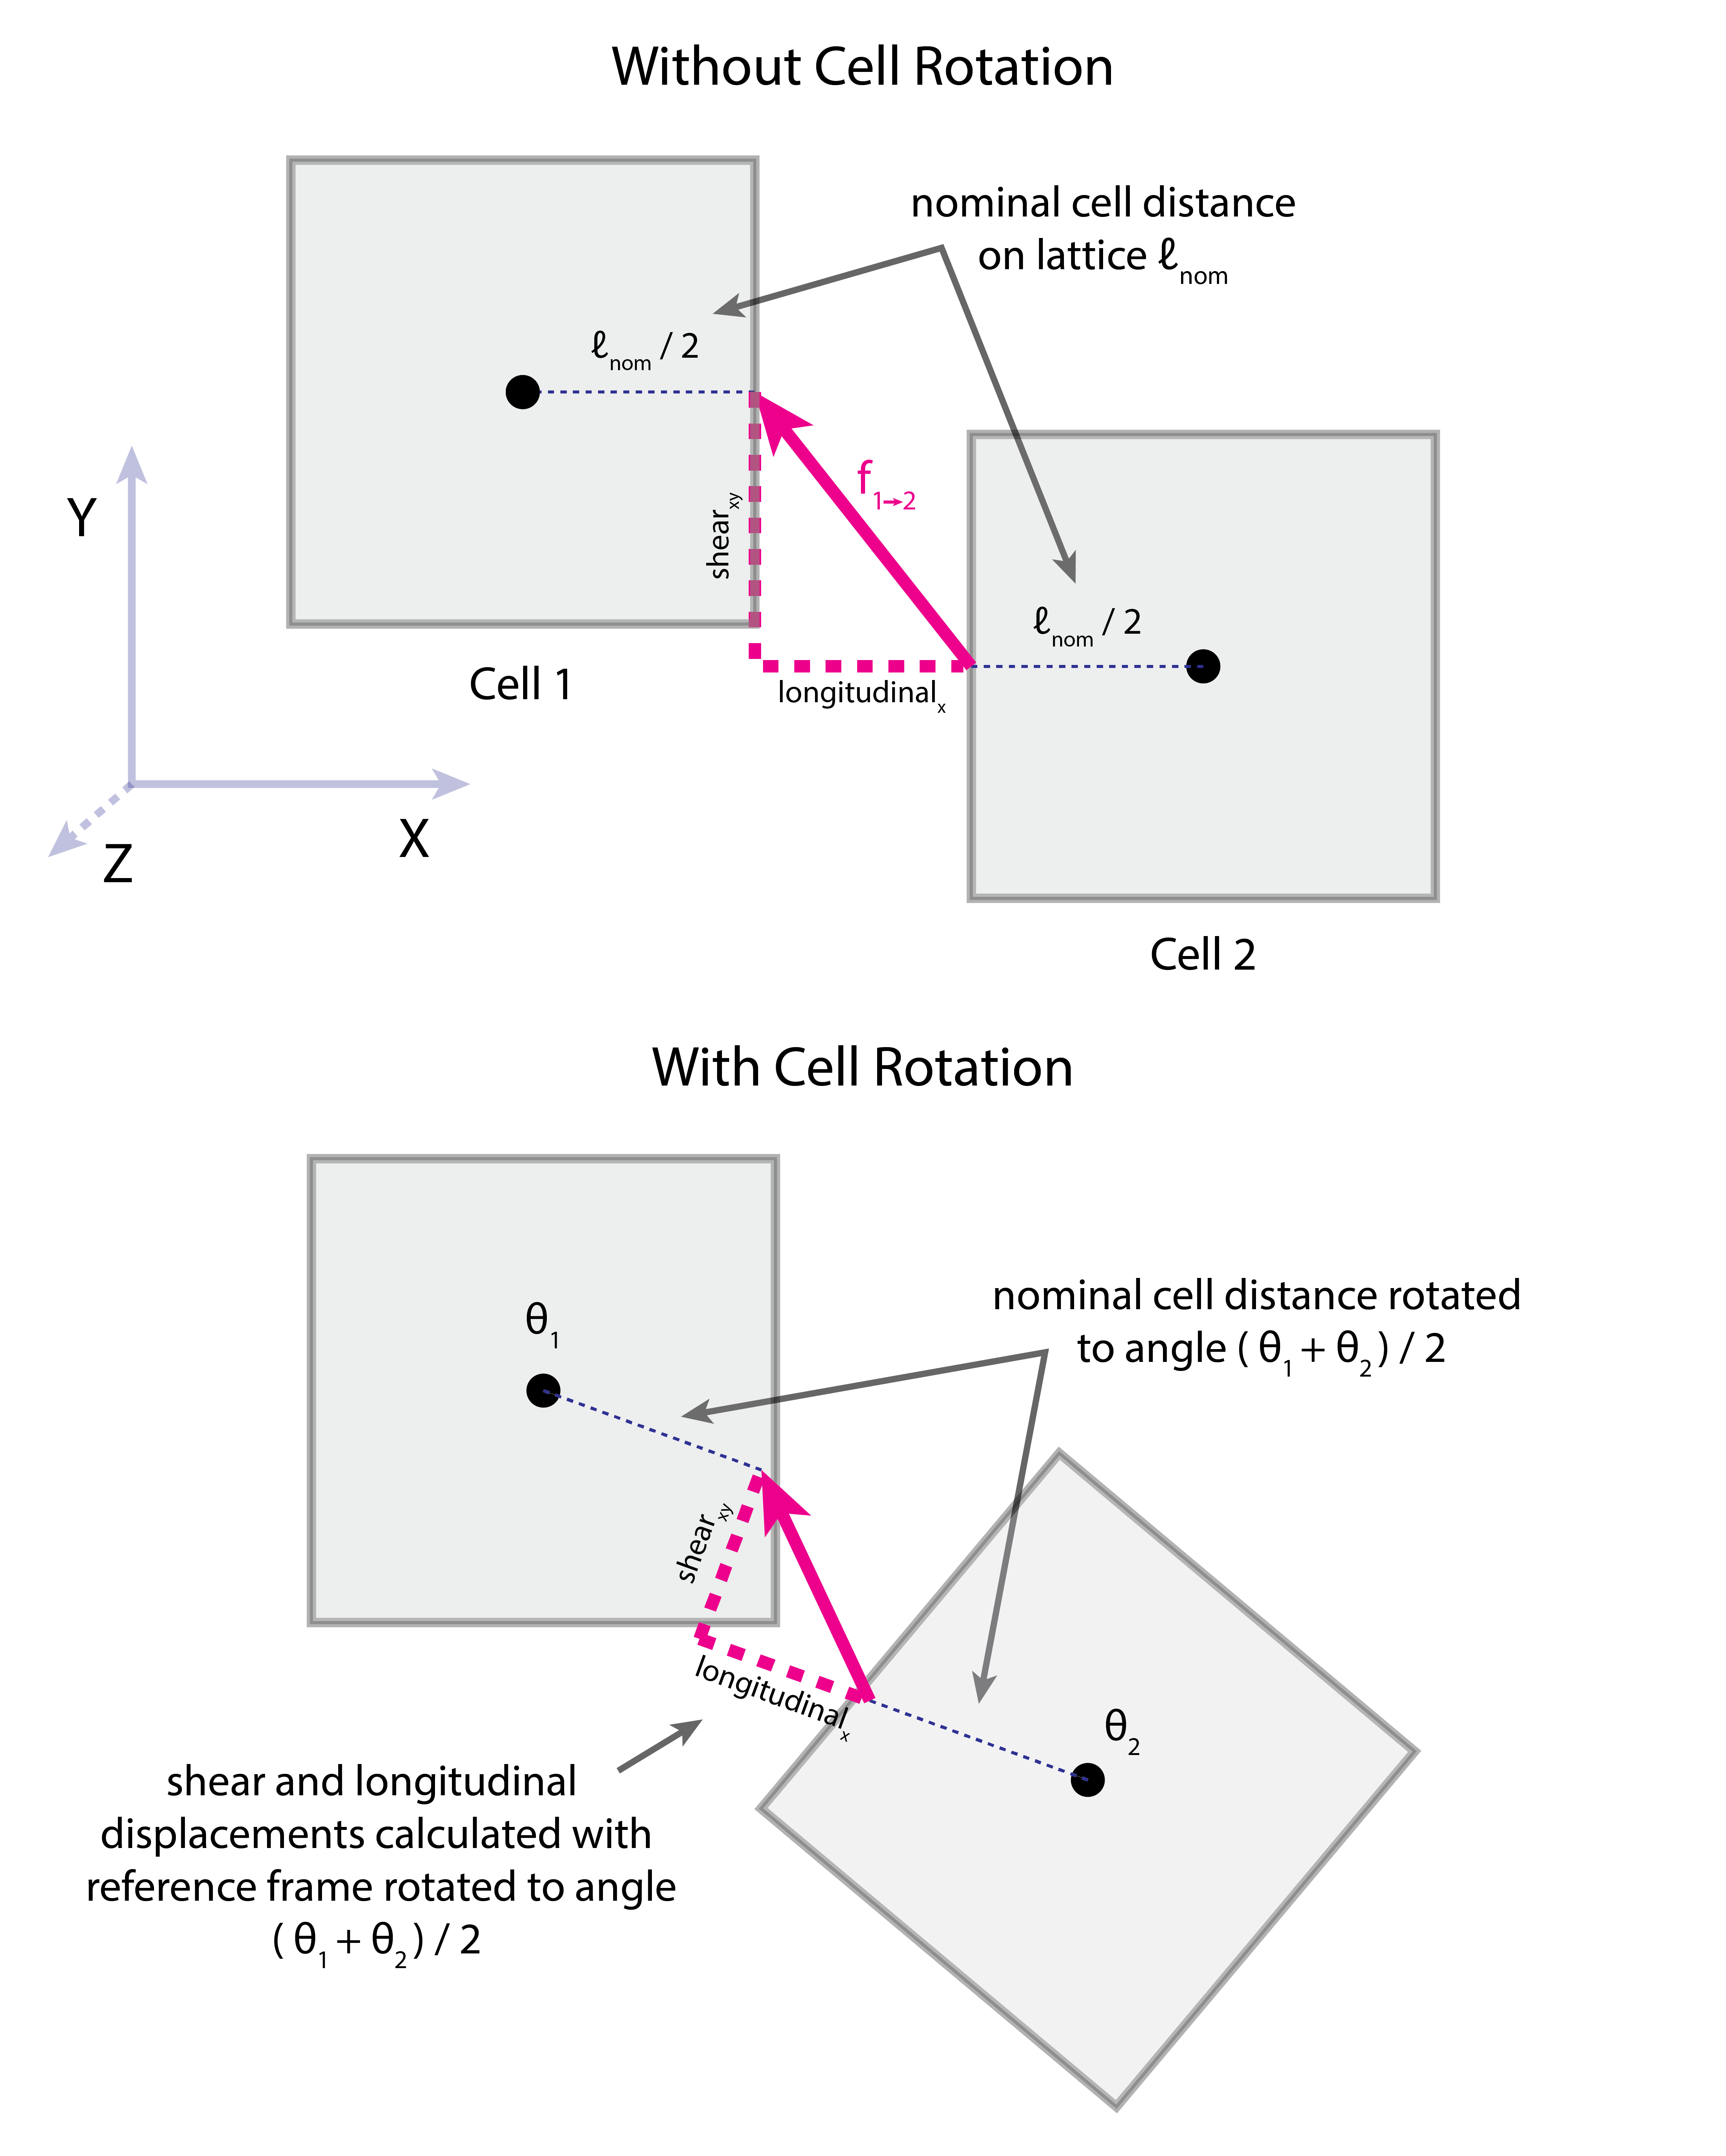
\includegraphics[width=\linewidth]{translationalSim.png}
  \caption{translationalSim.}
  \label{fig:translationalSim}
\end{figure}

In the simplest case without rotation, the force $\vec{F}_{1 \rightarrow 2}$ applied to cell 2 by cell 1 is given by:
\begin{equation} \label{eq:translationalForce}
\vec{F}_{1\rightarrow2} = \vec{k} \circ (\vec{p}_1 - \vec{p}_2) + \vec{d} \circ (\vec{v}_1 - \vec{v}_2)
\end{equation}

where $\vec{p}_1$ and $\vec{p}_2$ are the displacements of cell 1 and cell 2 from their nominal position in the lattice, $\vec{v}_1$ and $\vec{v}_2$ are the cells' translational velocities, $\circ$ is multiplication of two vectors by element, and $\vec{k}$ and $\vec{d}$ are 3D vectors containing the appropriate composite stiffness and damping constants for the interaction between the cells.  For example, given the scenario illustrated in Figure \ref{fig:translationalSim}, where two cells are connected along the x axis, an axial constant should be used for displacements along x and shear constants should be used for displacements along y and z:
\[ \vec{k} =  \left[ \begin{array}{ccc}
k_{axial_x}\\
k_{shear_{xy}}\\
k_{shear_{xz}}
 \end{array} \right]  
  \qquad\qquad
  \vec{d} =  \left[ \begin{array}{ccc}
d_{axial_x}\\
d_{shear_{xy}}\\
d_{shear_{xz}}
 \end{array} \right] \] 
 
If we wish to consider the orientations of the cells, denoted by the unit quaternions $q1$ and $q2$, we will need to adjust equation \ref{eq:translationalForce}. \\
  
  We can rotate a vector $\vec{v}$ in 3-space by a quaternion $q$ in 4-space:
    \[ \vec{v}_{rotated} = q*\vec{v}*q^* \]
  by treating $\vec{v}$ as a 4-space vector $[x, y, z, w]$ with $w=0$.  The operator $*$ denotes the Hamilton product:
  \[ a*b =  \left[ \begin{array}{ccc}
a_wb_x + a_xb_w + a_yb_z - a_zb_y\\
a_wb_y - a_xb_z + a_yb_w + a_zb_x\\
a_wb_z + a_xb_y - a_yb_x + a_zb_w\\
a_wb_w - a_xb_x - a_yb_y - a_zb_z
 \end{array} \right] \] 
 
   and $q^*$ denotes the conjugate of $q$:
    \[ q^{*} =  \left[ \begin{array}{ccc}
-q_x\\
-q_y\\
-q_z\\
q_w
 \end{array} \right] \] 
 
By performing a spherical linear interpolation (slerp) halfway between $q1$ and $q2$, we can calculate the average orientation of the two cells as a unit quaternion:
  \[ q_{avg} = slerp(q_{1}, q_{2}; 0.5) \]
  
Using $q_{avg}$, we can rotate the stiffness and damping vectors from Equation \ref{eq:translationalForce} into this average reference frame, and substitute the rotated vectors back into equation \ref{eq:translationalForce}:
 \[ \vec{k}_{rot} = (q_{avg}*\vec{k}*q_{avg}^*)\]
  \[ \vec{d}_{rot} = (q_{avg}*\vec{d}*q_{avg}^*)\]
  \begin{equation} \label{eq:translationalForceRotStep}
 \vec{F}_{1\rightarrow2} = \vec{k}_{rot} \circ (\vec{p}_1 - \vec{p}_2) + \vec{d}_{rot} \circ (\vec{v}_1 - \vec{v}_2)
 \end{equation}
 
Finally, we need to make an adjustment to the nominal differential position between the cells, indicated in Figure \ref{fig:translationalSim}.  The form above assumes the nominal distance between the centers of the cells is the unrotated distance from cells 2 to cell 1 in their initial lattice configuration, $\vec{l}_{nom21}$:
 \[\vec{l}_{nom21} = \vec{p}_{abs2}-\vec{p}_{abs1}\]
 
 where $\vec{p}_{abs}$ is the absolute position of a cell in the world reference frame.
 Rotating $\vec{l}_{nom}$ into the average rotational reference frame of the two cells gives
 \[\vec{l}_{rot21} = q_{avg}*\vec{l}_{nom21}*q_{avg}^*\]
 
introducing this correction to Equation \ref{eq:translationalForceRotStep} gives the final form:
 \begin{equation} \label{eq:translationalForceRot}
  \vec{F}_{1\rightarrow2} = \vec{k}_{rot} \circ (\vec{p}_1 - \vec{p}_2 + \vec{l}_{nom21}-\vec{l}_{rot21}) + \vec{d}_{rot} \circ (\vec{v}_1 - \vec{v}_2)
  \end{equation}

The force $\vec{F}_{2\rightarrow1}$ exerted on cell 2 by cell 1 is equal in magnitude to $\vec{F}_{1\rightarrow2}$ and opposite in direction:
 \begin{equation} \label{eq:translationalEqOpp}
  \vec{F}_{2\rightarrow1} = -\vec{F}_{1\rightarrow2} = \vec{k}_{rot} \circ (\vec{p}_1 - \vec{p}_2 + \vec{l}_{nom12}-\vec{l}_{rot12}) + \vec{d}_{rot} \circ (\vec{v}_1 - \vec{v}_2)
  \end{equation}

Only $\vec{F_{1\rightarrow2}}$ is indicated with a solid pink arrow in Figure \ref{fig:translationalSim}.\\

Dividing by the mass, we can calculate the acceleration of cells 1 and 2 due to interactions between them:

 \[ \vec{a}_{1\rightarrow2} = \dfrac{\vec{F}_{1\rightarrow2}}{m_2} 
  \qquad\qquad
   \vec{a}_{2\rightarrow1} = \dfrac{\vec{F}_{2\rightarrow1}}{m_1} 
  \]

\section{Rotational Forces}

So far, this model uses shear and axial stiffness and damping constants to compute the translational interactions between neighboring cells in 3D.  In order to incorporate bending and torsional forces, we must develop a method of for cells to apply torques to one another.  These torques result in rotational motion of a cell about its center of mass.\\

\begin{figure}
  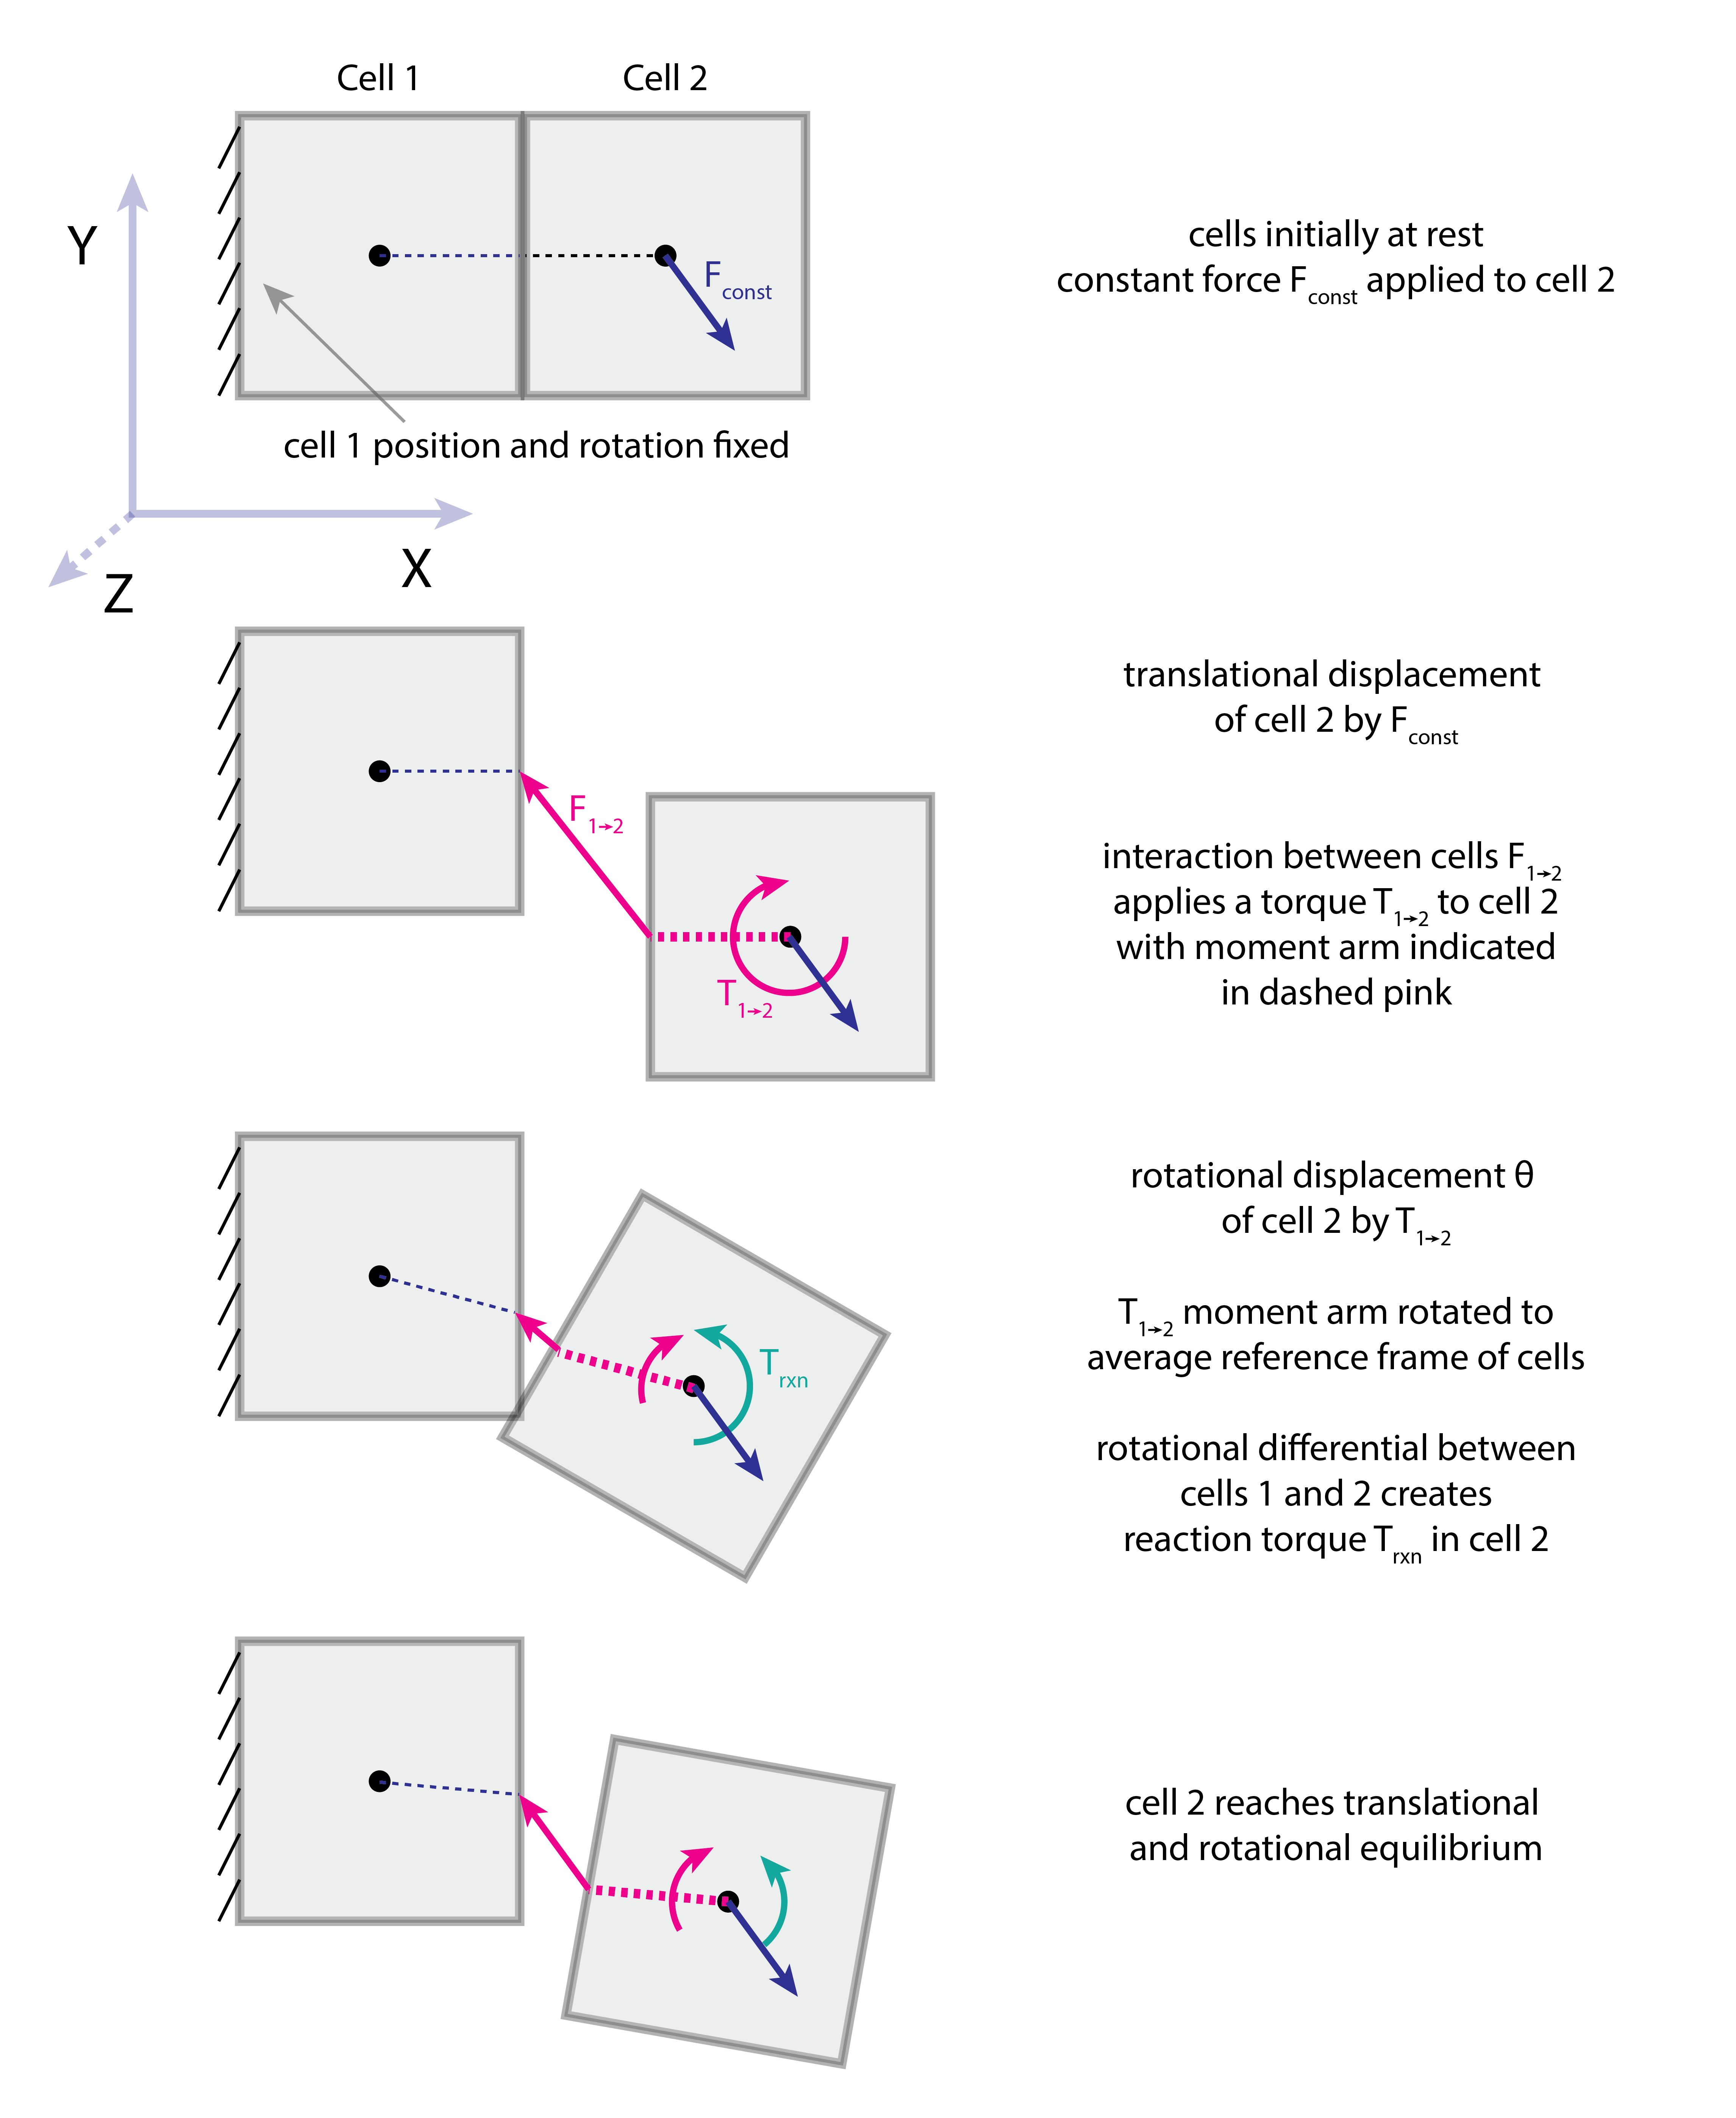
\includegraphics[width=\linewidth]{rotationalSim.png}
  \caption{rotationalSim}
  \label{fig:rotationalSim}
\end{figure}

A sketch of the translational and rotational model for cell interaction is shown in Figure \ref{fig:rotationalSim}.  In this model, we consider the fact that shear and axial forces between cells are not applied directly to the center of mass of a cell, but rather at some moment arm from the center of mass.  We define the moment arm $\vec{r}_{moment2}$ of cell 2 to be half the nominal distance from cell 2 to cell 1, rotated to the average reference frame of the two cells:

\[ \vec{r}_{moment} = \dfrac{\vec{l}_{rot21}}{2}\]

Then the torque $\vec{T}_{1\rightarrow2}$ can be calculated by the cross product:

\[ \vec{T}_{1\rightarrow2} =  \vec{r}_{moment} \times \vec{F}_{1\rightarrow2}\]

If we stop now, we have set up a simulation of an arbitrary linkage of cells tied together with frictionless, spherical joints at their centers of mass.  Figure -- shows a few times steps of this system under the force of gravity.\\

Next we'll add in bending and torsional stiffness, which create reaction forces that counteract relative rotations between cells ($T_{rxn}$ in Figure \ref{fig:rotationalSim}).  \\

\section{Comparison with Traditional FEA Techniques}

\begin{figure}
  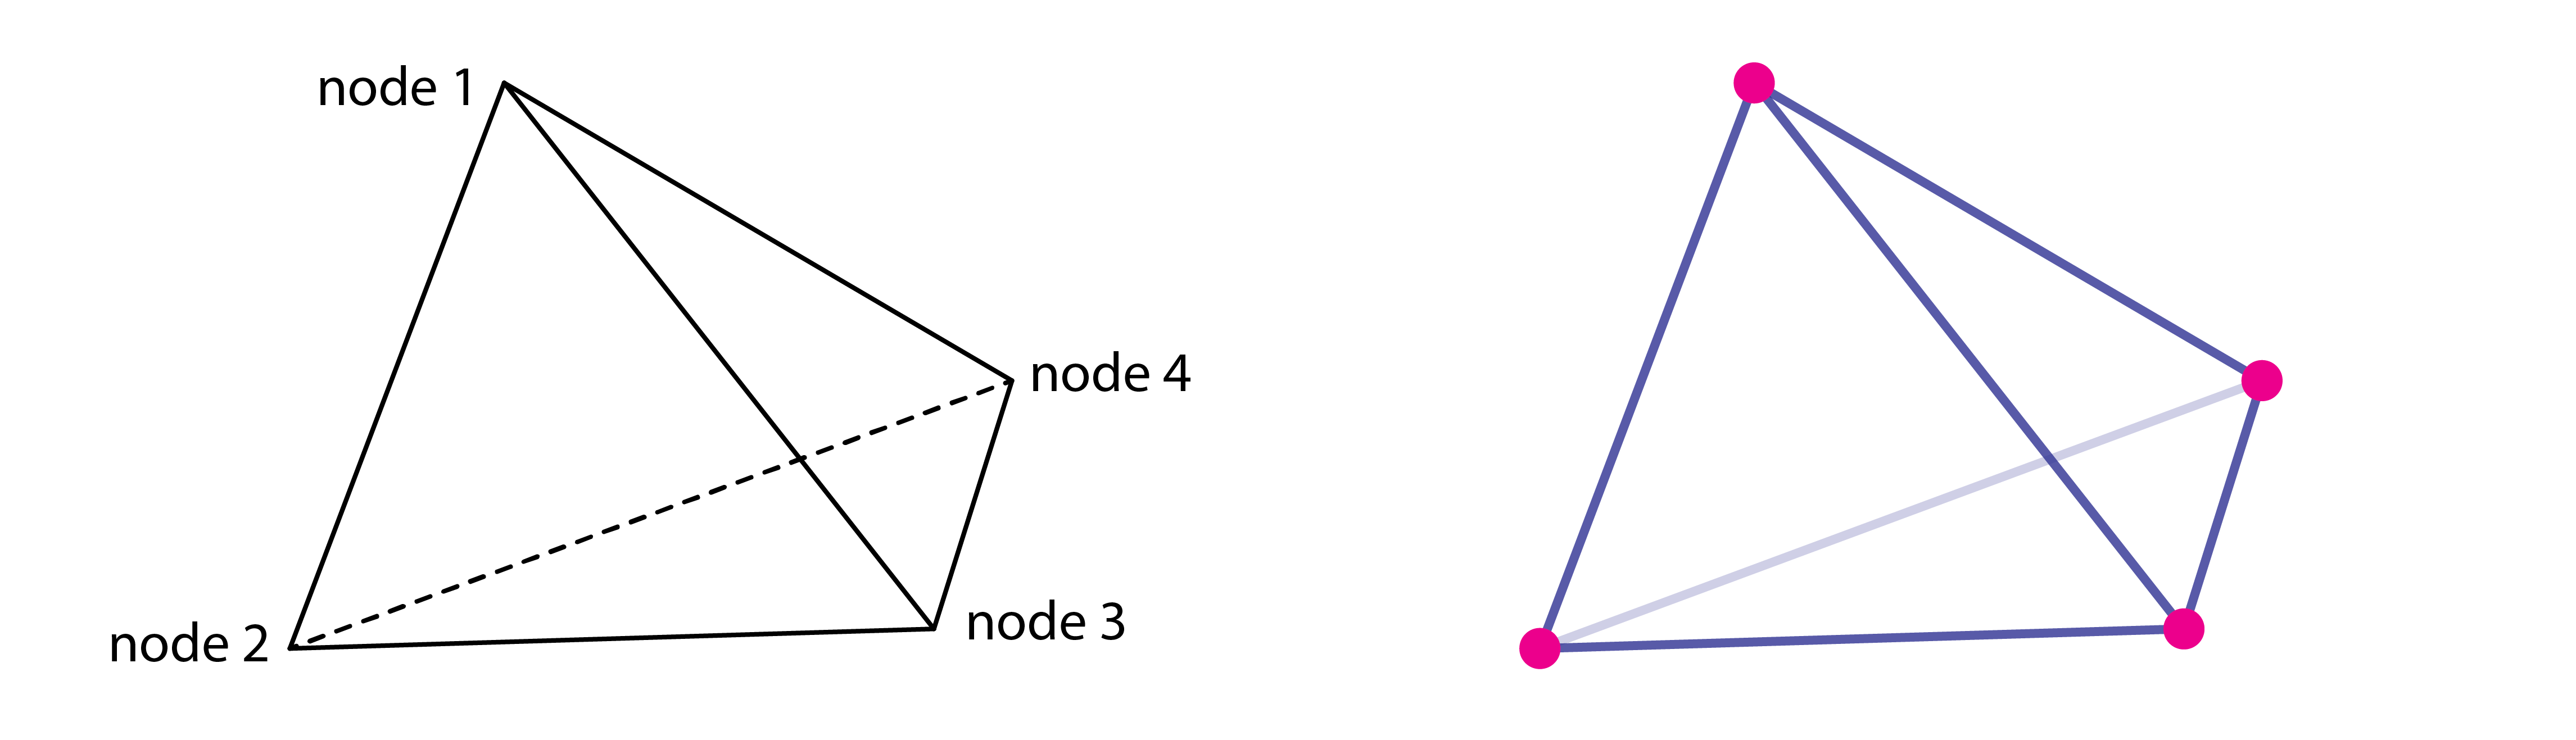
\includegraphics[width=\linewidth]{TetraElement.png}
  \caption{A tetrahedral element in 3D FEA.  The vertices of each element are called nodes.  In linear elastic solids, the relationships between forces (stress) and displacement (strain) of the nodes is described by variations on Hooke's law.  The springs indicated in the figure on the right are meant to illustrate the linear elastic (Hookian) relationship between nodes.  Typically, interactions between nodes are modeled with 6DOF linear elastic relationships as opposed to a 1DOF spring.}
  \label{fig:TetraElement}
\end{figure}

Following from Figure \ref{fig:FEAexample}, the basic idea behind FEA of linear elastic solids is to break up geometry into many small \textit{finite elements} whose behavior can be closely approximated by Hooke's law.  In 3D, these elements might have any number of shapes, a common element shape is the tetrahedral illustrated in Figure \ref{fig:TetraElement}.\\

The vertices of each finite element are called nodes.  Nodes connect to other nodes through the edges of the elements to form a mesh.  No assumptions are made about the length of the edges of a finite element; in fact one of the main advantages of FEA is the ability to locally alter the resolution of the mesh in a particular region of interest.\\

\textit{Shape functions} are polynomials in 1D, 2D, or 3D that describe how the behavior of the nodes should be interpolated in the regions between the nodes (eg the inner volume of the tetrahedron in Figure \ref{fig:TetraElement}).  Hermitian cubic shape functions are typically used for beam models; they are third order polynomials that provide continuity between discretized solutions along nodes in a beam.  A graphical description of shape functions is shown in Wolfram \cite{Wolfram2016}.  The shape functions expressed in terms of a dimensionless coordinate $\xi$ are:
\begin{align*} 
N_{x1} &= \textstyle\frac{1}{4}(1-\xi)^2(2+\xi)\\
N_{x2} &= \textstyle\frac{1}{4}(1+\xi)^2(2-\xi)\\
N_{\theta1} &= \textstyle\frac{1}{8}l(1-\xi)^2(1+\xi)\\
N_{\theta2} &= \textstyle\frac{1}{8}l(1+\xi)^2(1-\xi)
\end{align*}

where $-1 \leq \xi \leq 1$ and $\xi = -1$ at node 1 and $\xi = 1$ at node 2\\

Using these shape functions we can calculate the \textit{stiffness matrix} ($K$) of a beam element.  


\begin{figure}
  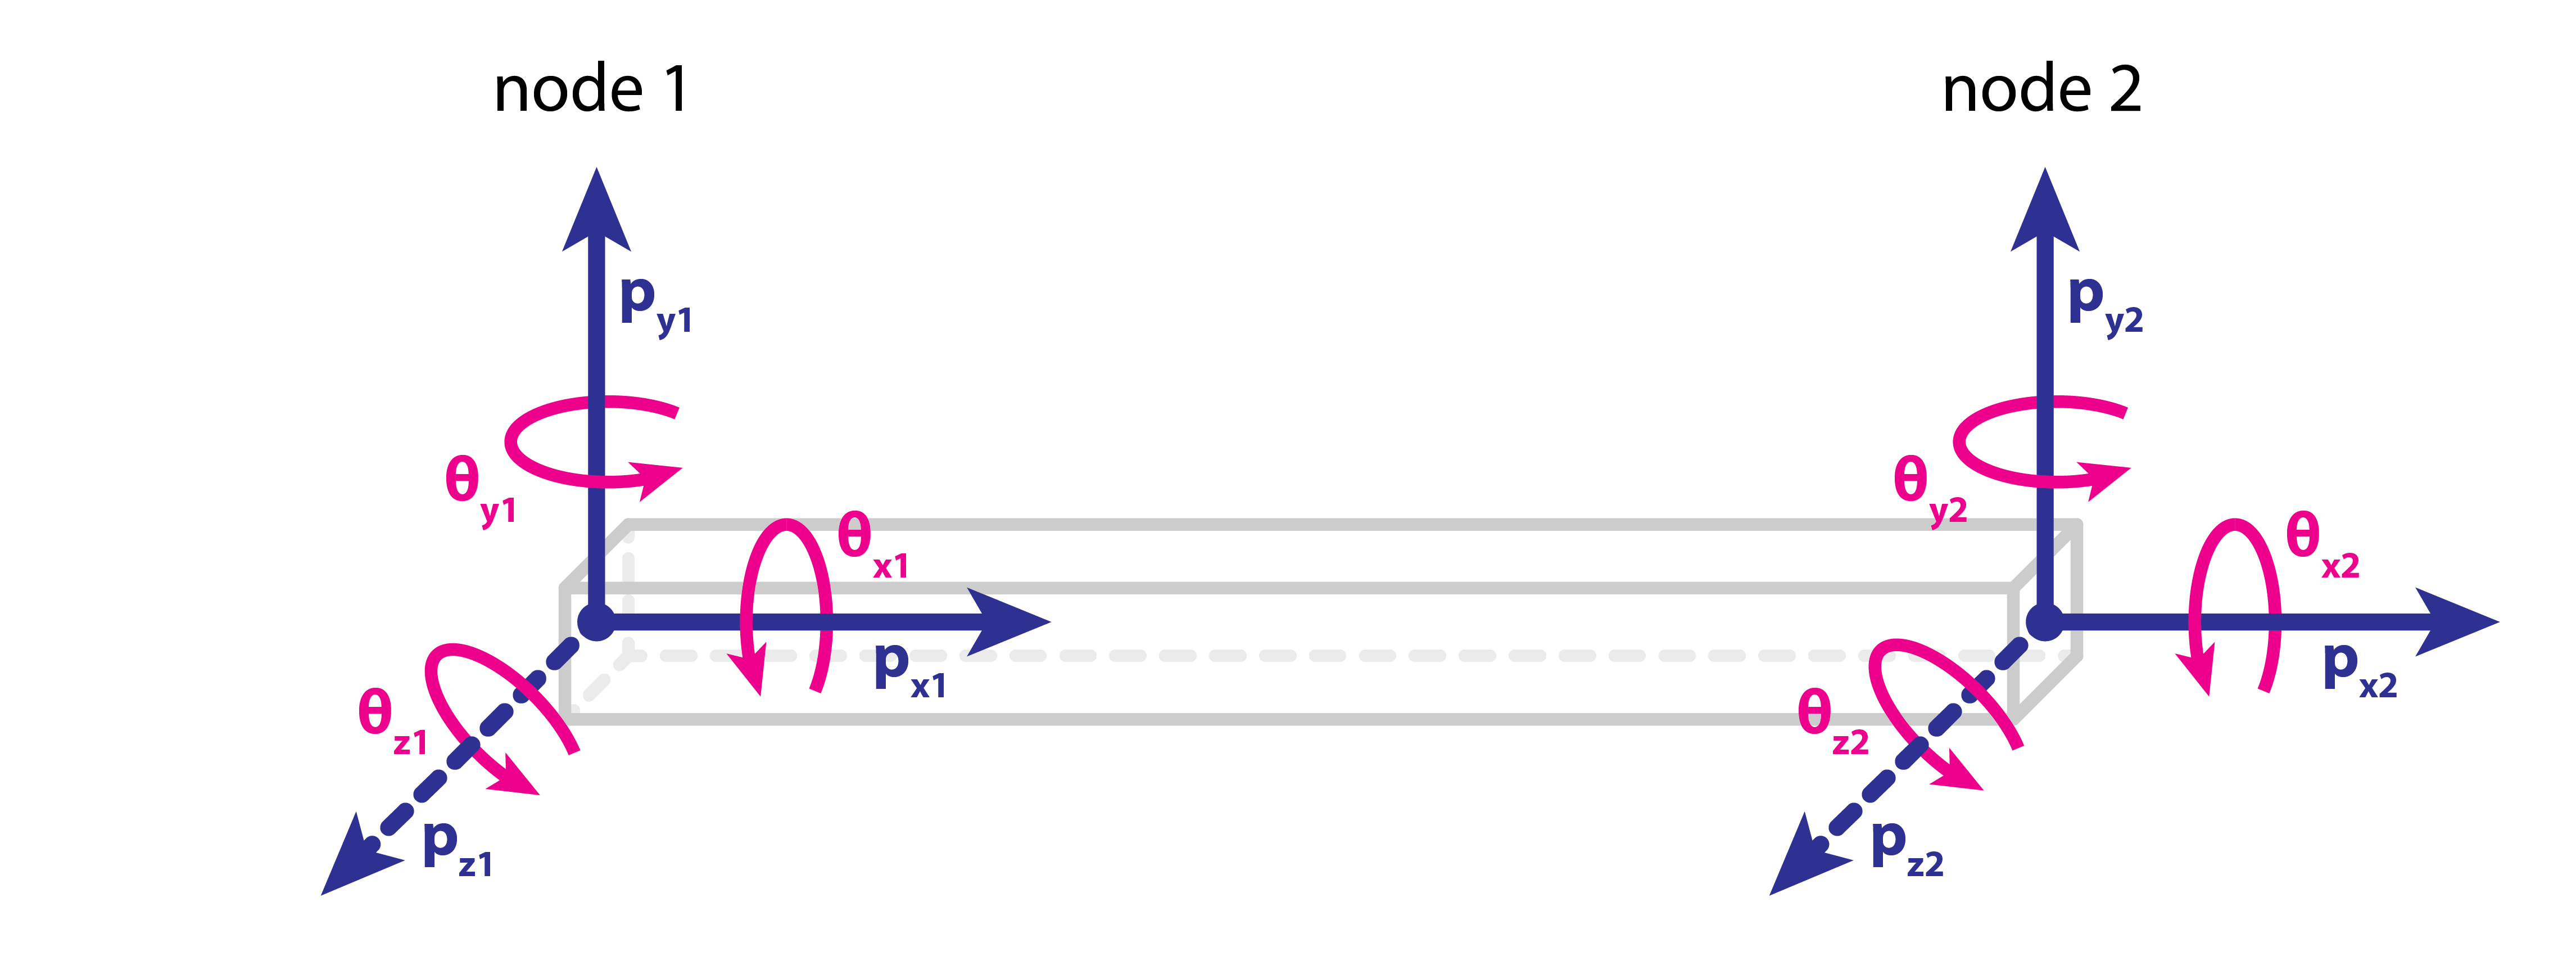
\includegraphics[width=\linewidth]{BeamSetup.png}
  \caption{Setup of 12DOF beam model connecting two nodes (nodes 1 and 2).  Translational displacement indicated by $p_x$, $p_y$, $p_z$ and angular displacement indicated by $\theta_x$, $\theta_y$, $\theta_z$.}
  \label{fig:BeamSetup}
\end{figure}

The Timoshenko beam element takes into account axial deformation, bending deformations in the orthogonal direction with shear effects, and torsional deformation.  A 12DOF Timoshenko beam oriented along the x-axis has the stiffness matrix:\\

\[ K =  \scriptsize {\left[ \begin{smallmatrix}
\tfrac{EA}{l} & 0 & 0 & 0 & 0 & 0 & \tfrac{-EA}{l} & 0 & 0 & 0 & 0 & 0\\
 & \tfrac{12EI_z}{l^3(1+\phi_y)} & 0 & 0 & 0 & \tfrac{6EI_z}{l^2(1+\phi_y)} & 0 & \tfrac{-12EI_z}{l^3(1+\phi_y)} & 0 & 0 & 0 & \tfrac{6EI_z}{l^2(1+\phi_y)}\\
 &  & \tfrac{12EI_y}{l^3(1+\phi_z)} & 0 & \tfrac{-6EI_y}{l^2(1+\phi_z)} & 0 & 0 & 0 & \tfrac{-12EI_y}{l^3(1+\phi_z)} & 0 & \tfrac{-6EI_y}{l^2(1+\phi_z)} & 0\\
 &  &  &  \tfrac{GJ}{l} &  0 &  0 &  0 &  0 &  0 & \tfrac{-GJ}{l} & 0 & 0\\
 &  &  &  & \tfrac{(4+\phi_z)EI_y}{l(1+\phi_z)} & 0 & 0 & 0 & \tfrac{6EI_y}{l^2(1+\phi_z)} & 0 & \tfrac{(2-\phi_z)EI_y}{l(1+\phi_z)} & 0\\
 &  &  &  &  & \tfrac{(4+\phi_y)EI_z}{l(1+\phi_y)} & 0 & \tfrac{-6EI_z}{l^2(1+\phi_y)} & 0 & 0 & 0 & \tfrac{(2-\phi_y)EI_z}{l(1+\phi_y)}\\
 &  &  &  &  &  & \tfrac{EA}{l}  & 0 & 0 & 0 & 0 & 0\\
 &  &  &  &  &  &  & \tfrac{12EI_z}{l^3(1+\phi_y)} & 0 & 0 & 0 & \tfrac{-6EI_z}{l^2(1+\phi_y)}\\
 &  &  &  &  &  &  &  & \tfrac{12EI_y}{l^3(1+\phi_z)} & 0 & \tfrac{6EI_y}{l^2(1+\phi_z)}\ & 0\\
 &  & symmetric &  &  &  &  &  &  & \tfrac{GJ}{l} & 0 & 0\\
 &  &  &  &  &  &  &  &  &  & \tfrac{(4+\phi_z)EI_y}{l(1+\phi_z)} & 0\\
  &  &  &  &  &  &  &  &  &  &  & \tfrac{(4+\phi_y)EI_z}{l(1+\phi_y)}\\
 \end{smallmatrix} \right] }\]
 
 where
\[ \phi_y = \dfrac{12EI_z}{GA_{sy}l^2} \qquad  \textrm{and} \qquad \phi_z = \dfrac{12EI_y}{GA_{sz}l^2} \]


The stiffness matrix gives us a way to convert between translational/rotational nodal displacements and forces, according to the following equation:

 \begin{equation} \label{eq:forcestiffnessdisp} \vec{F} = K\vec{u} \end{equation}
where:
\[ \vec{F} =  \left[ \begin{array}{ccc}
F_{x1}\\
F_{y1}\\
F_{z1}\\
T_{x1}\\
T_{y1}\\
T_{z1}\\
F_{x2}\\
F_{y2}\\
F_{z2}\\
T_{x2}\\
T_{y2}\\
T_{z2}
 \end{array} \right]  \qquad \qquad  
 \vec{u} =  \left[ \begin{array}{ccc}
p_{x1}\\
p_{y1}\\
p_{z1}\\
\theta_{x1}\\
\theta_{y1}\\
\theta_{z1}\\
p_{x2}\\
p_{y2}\\
p_{z2}\\
\theta_{x2}\\
\theta_{y2}\\
\theta_{z2}
 \end{array} \right]
 \]\\
 
where $F_1$, $F_2$ are translational forces on nodes 1 and 2, $T$ are torques, $p$ are translational positions, and $\theta$ are rotations.\\

Multiplying through Equation \ref{eq:forcestiffnessdisp} gives us 12 equations:

\begin{subequations}
\begin{align} 
\label{eq:fx1}
F_{x1} &=  \dfrac{EA}{l}p_{x1} - \dfrac{EA}{l}p_{x2} \\[10pt]
\label{eq:fy1}
F_{y1} &=  \dfrac{12EI_z}{l^3(1+\phi_y)}p_{y1} + \dfrac{6EI_z}{l^2(1+\phi_y)}\theta_{z1} - \dfrac{12EI_z}{l^3(1+\phi_y)}p_{y2} + \dfrac{6EI_z}{l^2(1+\phi_y)}\theta_{z2}\\[10pt]
\label{eq:fz1}
F_{z1} &=  \dfrac{12EI_y}{l^3(1+\phi_z)}p_{z1} - \dfrac{6EI_y}{l^2(1+\phi_z)}\theta_{y1} - \dfrac{12EI_y}{l^3(1+\phi_z)}p_{z2} - \dfrac{6EI_y}{l^2(1+\phi_z)}\theta_{y2}\\[10pt]
\label{eq:tx1}
T_{x1} &=  \dfrac{GJ}{l}\theta_{x1} - \dfrac{GJ}{l}\theta_{x2} \\[10pt]
\label{eq:ty1}
T_{y1} &= - \dfrac{6EI_y}{l^2(1+\phi_z)}p_{z1} + \dfrac{(4+\phi_z)EI_y}{l(1+\phi_z)}\theta_{y1}  + \dfrac{6EI_y}{l^2(1+\phi_z)}p_{z2} + \dfrac{(2-\phi_z)EI_y}{l(1+\phi_z)}\theta_{y2} \\[10pt]
\label{eq:tz1}
T_{z1} &=  \dfrac{6EI_z}{l^2(1+\phi_y)}p_{y1} + \dfrac{(4+\phi_y)EI_z}{l(1+\phi_y)}\theta_{z1}  - \dfrac{6EI_z}{l^2(1+\phi_y)}p_{y2} + \dfrac{(2-\phi_y)EI_z}{l(1+\phi_y)}\theta_{z2} \\[10pt]
\label{eq:fx2}
F_{x2} &=  -F_{x1}\\[10pt]
\label{eq:fy2}
F_{y2} &=  -F_{y1}\\[10pt]
\label{eq:fz2}
F_{z2} &=  -F_{z1}\\[10pt]
\label{eq:tx2}
T_{x2} &=  -T_{x1}\\[10pt]
\label{eq:ty2}
T_{y2} &=  - \dfrac{6EI_y}{l^2(1+\phi_z)}p_{z1} + \dfrac{(2+\phi_z)EI_y}{l(1+\phi_z)}\theta_{y1}  + \dfrac{6EI_y}{l^2(1+\phi_z)}p_{z2} + \dfrac{(4-\phi_z)EI_y}{l(1+\phi_z)}\theta_{y2} \\[10pt]
\label{eq:tz2}
T_{z2} &= \dfrac{6EI_z}{l^2(1+\phi_y)}p_{y1} + \dfrac{(2+\phi_y)EI_z}{l(1+\phi_y)}\theta_{z1}  - \dfrac{6EI_z}{l^2(1+\phi_y)}p_{y2} + \dfrac{(4-\phi_y)EI_z}{l(1+\phi_y)}\theta_{z2}
\end{align}
\end{subequations}\\

Combining Equations \ref{eq:fx1} and \ref{eq:kaxial} gives us the x-axis spring component of Equation \ref{eq:translationalForceRot}, assuming no relative rotation between the nodes:
\[F_{x1} =  k_{axial_x}(p_{x1} - p_{x2}) \]\\

Equations \ref{eq:fy1} and \ref{eq:fz1} have essentially the same form.  Rearranging Equation \ref{eq:fy1} gives:
\[ F_{y1} =  \dfrac{12EI_z}{l^3(1+\phi_y)} (p_{y1} -p_{y2}) + \dfrac{6EI_z}{l^2(1+\phi_y)}(\theta_{z1} + \theta_{z2}) \]\\

Combining Equations \ref{eq:tz1} and \ref{eq:ktorsion} gives us the x-axis rotational component of Equation ---
\[T_{x1} =  k_{torsion_x}(\theta_{x1} - \theta_{x2}) \]\\

As discussed in Equation \ref{eq:translationalEqOpp}, the translational forces acting on node 1 are equal and opposite those acting on node 2.  This is summed up by Equations \ref{eq:fx2}, \ref{eq:fy2}, and \ref{eq:fz2}.  This \\

Removing the shear terms from elements of the 12DOF Timoshenko stiffness matrix gives the Euler-Bernoulli beam theory (only valid for small angle approx)\\


\[ K =  \small {\left[ \begin{smallmatrix}
\tfrac{EA}{l} & 0 & 0 & 0 & 0 & 0 & \tfrac{-EA}{l} & 0 & 0 & 0 & 0 & 0\\
 & \tfrac{12EI_z}{l^3} & 0 & 0 & 0 & \tfrac{6EI_z}{l^2} & 0 & \tfrac{-12EI_z}{l^3} & 0 & 0 & 0 & \tfrac{6EI_z}{l^2}\\
 &  & \tfrac{12EI_y}{l^3} & 0 & \tfrac{-6EI_y}{l^2} & 0 & 0 & 0 & \tfrac{-12EI_y}{l^3} & 0 & \tfrac{-6EI_y}{l^2} & 0\\
 &  &  &  \tfrac{GJ}{l} &  0 &  0 &  0 &  0 &  0 & \tfrac{-GJ}{l} & 0 & 0\\
 &  &  &  & \tfrac{4EI_y}{l} & 0 & 0 & 0 & \tfrac{6EI_y}{l^2} & 0 & \tfrac{EI_y}{l} & 0\\
 &  &  &  &  & \tfrac{4EI_z}{l} & 0 & \tfrac{-6EI_z}{l^2} & 0 & 0 & 0 & \tfrac{EI_z}{l}\\
 &  &  &  &  &  & \tfrac{EA}{l}  & 0 & 0 & 0 & 0 & 0\\
 &  &  &  &  &  &  & \tfrac{12EI_z}{l^3} & 0 & 0 & 0 & \tfrac{-6EI_z}{l^2}\\
 &  &  &  &  &  &  &  & \tfrac{12EI_y}{l^3} & 0 & \tfrac{6EI_y}{l^2}\ & 0\\
 &  & symmetric &  &  &  &  &  &  & \tfrac{GJ}{l} & 0 & 0\\
 &  &  &  &  &  &  &  &  &  & \tfrac{4EI_y}{l} & 0\\
  &  &  &  &  &  &  &  &  &  &  & \tfrac{4EI_z}{l}\\
 \end{smallmatrix} \right] } \]

\section{Sources of Error}

\begin{figure}
  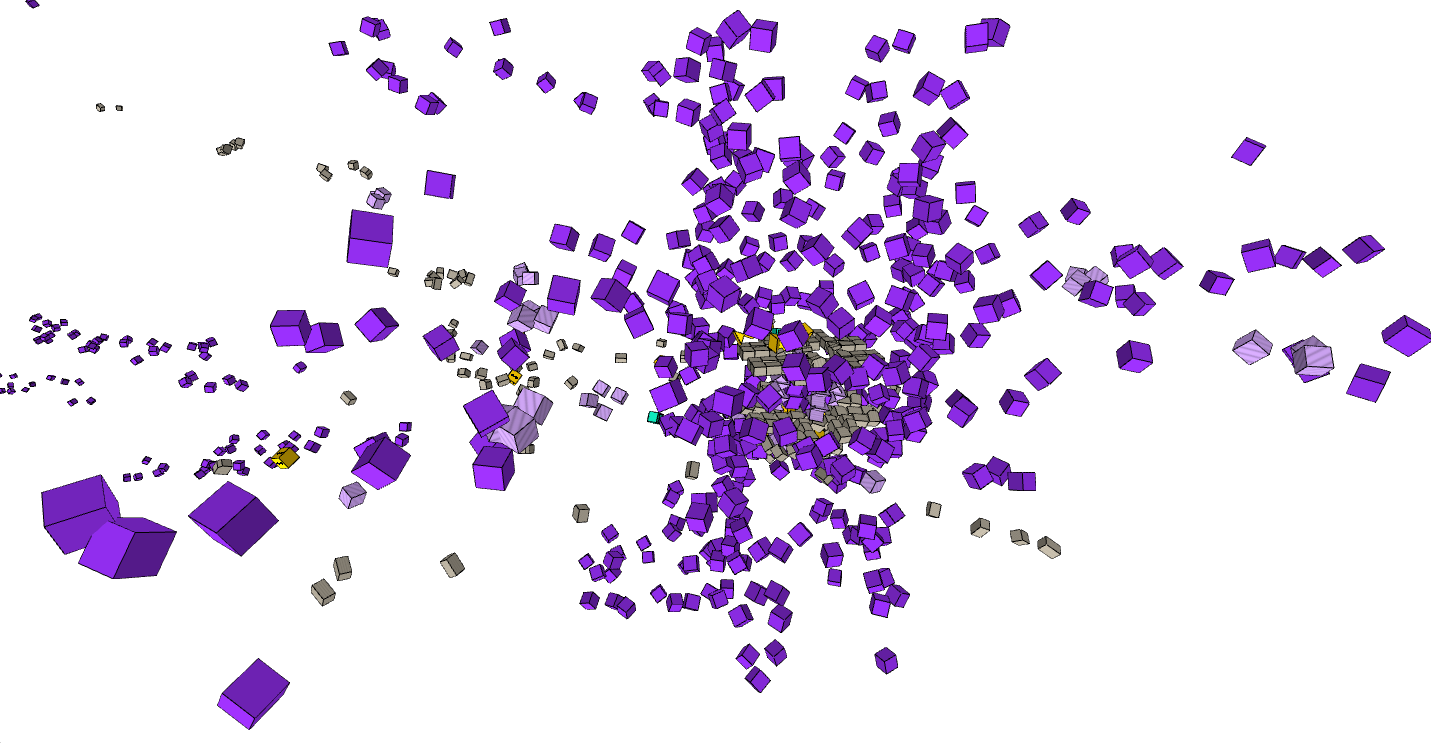
\includegraphics[width=\linewidth]{instability.png}
  \caption{instability.png.}
  \label{fig:instability}
\end{figure}

\subsection{Numerical Time Integration}

For linear systems, explicit forward time integration can be achieved using a variety of methods, each with associated error and computational cost.  The simplest and most computationally efficient approach is forward Euler:
\[ \vec{v}_{t+1} = \vec{v}_{t} +  \vec{a}_{t}\Delta t\]
\[ \vec{p}_{t+1} = \vec{p}_{t} +  \vec{v}_{t}\Delta t\]

Verlet integration requires storing the previous two position calculations (at time $t$ and $t-1$) in order to calculate the next position:
\[ \vec{p}_{t+1} = 2\vec{p}_{t} - \vec{p}_{t-1} +  \vec{a}_{t}\Delta t^2\]
\[ \vec{v}_{t+1} = \dfrac{\vec{p}_{t+1} - \vec{p}_{t}}{\Delta t}\]

Higher order methods such as Runge-Kutta (RK4) reduce error further, but require multiple calculations in order to solve for a single time step.

rotational case
\[ \vec{\omega}_{t+1} = \vec{\omega}_{t} +  \vec{\alpha}_{t}\Delta t\]
\[ \dot{q} = 1/2\vec{\omega}*q\]
again, with $\vec{\omega}$ as a 4-space vector with $w=0$ and $*$ denoting the Hamilton product.

\subsection{Floating Point Operations}

\section{Electronic Simulation}\label{sec:electronicSim}

\section{Hierarchical Simulation}

\section{Performance Speedups}

A faster method of applying quaternions to vectors is given by
\[ t = 2 \left[ \begin{array}{ccc}
q_x\\
q_y\\
q_z
 \end{array} \right] \times v\]
\[ v_{rotated} = v + q_wt +  \left[ \begin{array}{ccc}
q_x\\
q_y\\
q_z
 \end{array} \right] \times t\]
 https://blog.molecular-matters.com/2013/05/24/a-faster-quaternion-vector-multiplication/


\section{Deviations from Reality}

\subsection{Volume Preservation}

Poisson's ratio $v$

\begin{figure}
  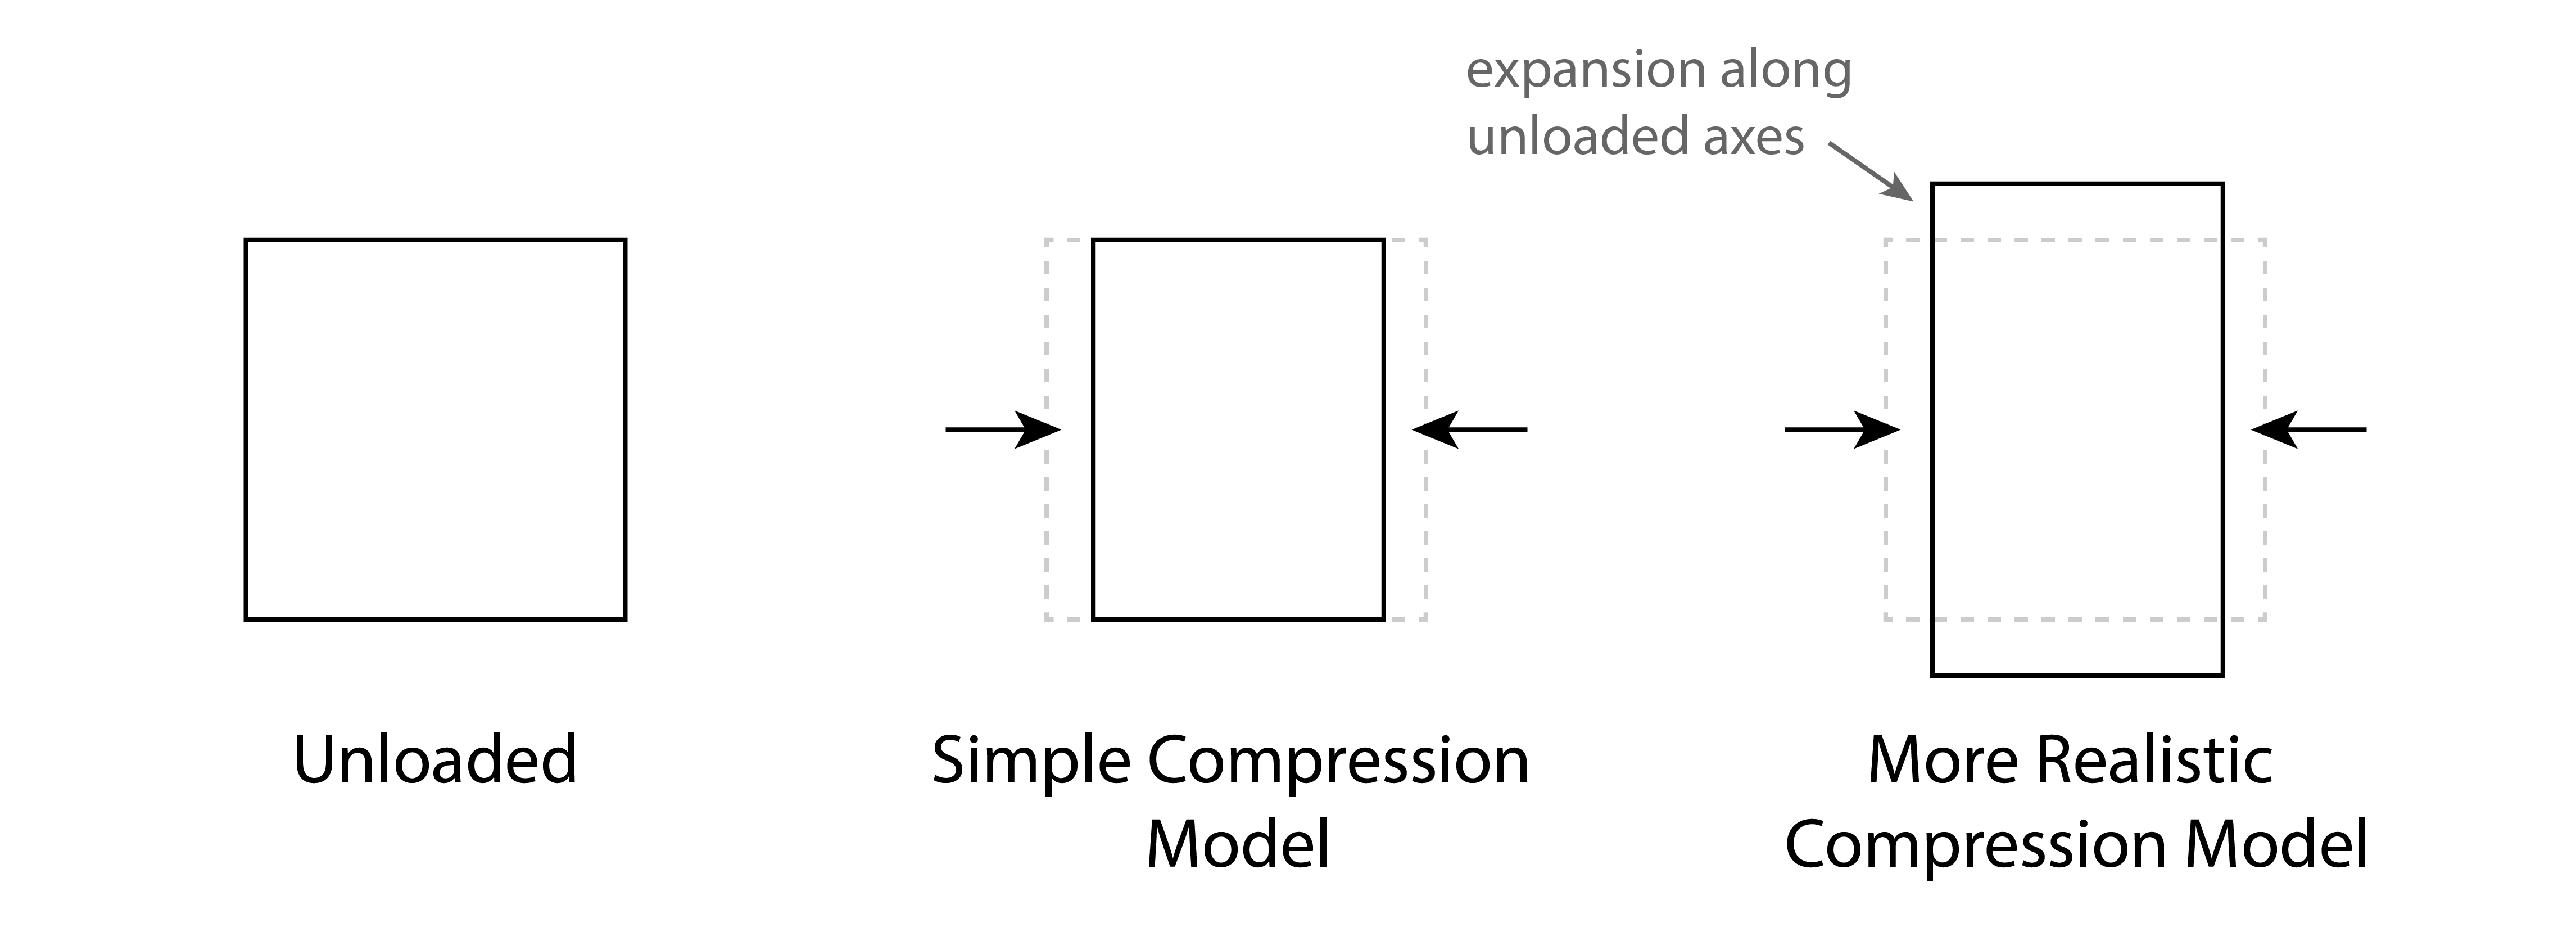
\includegraphics[width=\linewidth]{SolidMechanicsReality.png}
  \caption{Deviation from reality in simple \textit{function} simulation.  Some coupling between degrees of freedom is expected, for example, compression on one axis will result in expansion along other, unloaded axes.}
  \label{fig:SolidMechanicsReality}
\end{figure}

In reality, the degrees of freedom illustrated in Fig \ref{fig:SolidMechanicsDOF} are not completely orthogonal from one another.  For example, compression along one axis of a solid will cause some degree of expansion along the unloaded axes (Fig \ref{fig:SolidMechanicsReality}).


}
